\section{Appendix roadmap and evidence inventory}
\label{app:roadmap}

The appendix is organised by evidentiary role rather than by experiment
chronology. It starts with companion readouts, then documents primary
estimators, uncertainty, task-level sources, and estimator sensitivity. Middle
sections collect mechanism diagnostics and same-backbone perturbation analyses; later
sections cover adaptation, data swaps, segmentation-pipeline variants,
distribution shift, operational metrics, held-out stress tests, and
$M_{\text{eff}}$. The final sections record artifact metadata and additional
scope analyses. Secondary rows are retained only when they qualify or
explain a paper claim, and their captions state when they use non-primary pools
or splits. Unless explicitly marked primary or sourced from the primary
\texttt{results/\_merged} summaries, appendix values are diagnostic rather than
primary support for Table~\ref{tab:main}.

\paragraph{CLIP-L notation.}
Throughout the appendix, CLIP-L/14 refers to the preserved OpenCLIP
\texttt{ViT-L-14/openai} dense-token wrapper used to generate the released
traces. It is not a claim of OpenAI \texttt{clip.load} parity; a strict
QuickGELU-parity CLIP-L loader would be a separate sensitivity with a distinct
FM identifier.

\begin{table}[!htbp]
  \caption{\textbf{Appendix guide.} Each block has a single role in the
  argument; cross-references point to the detailed tables rather than repeating
  them in the main paper.}
  \label{tab:appendix-guide}
  \centering\footnotesize
  \begin{tabular}{p{0.24\linewidth}p{0.62\linewidth}}
    \toprule
    Block & Evidence role \\
    \midrule
    Estimators and provenance & Case/hierarchical bootstrap, subject clustering,
    quality-controlled pair regression, functional-floor/ICC/permutation sensitivity, pixel overlap,
    annotation-source note, and primary dataset details. \\
    Mechanism diagnostics & Same-architecture-family ViT / different-pretraining,
    CKA, random-effects, and
    item-difficulty null analyses. \\
    Same-backbone perturbation analyses & Matched-size/quality-gated pool checks, decoder capacity, UNet skips,
    fixed-backbone folds, MC dropout, released CNN random-init, and labelled scope-limited probes. \\
    Scope boundaries & nnU-Net complements, 3D pilot, BraTS sparse-target
    sensitivities, loss/augmentation sensitivity, distribution shift, and held-out failures. \\
    Operational metrics & Conditional recovery, matched-$M$ lift, lift ceiling,
    pool-selection probes, and $M_{\text{eff}}$. \\
    Artifact documentation & Bundle manifest, artifact metadata, requirements, and
    trace inventory. \\
    \bottomrule
  \end{tabular}
\end{table}

\section{Companion readouts and scope}
\label{sec:cka}
\label{app:per-rater}
\label{sec:confidence-app}

This section records companion readouts that clarify scope without adding new
headline claims.

\textbf{CKA.} We computed CKA only as a descriptive feature-similarity readout.
The saved partial-regression coefficient artifact is not included in the
supplementary artifact, so we do not use partial-regression $p$-values or coefficients
as formal evidence. The main paper relies on pixel-level failure overlap and
per-case Dice correlation for mechanism-adjacent interpretation, and treats CKA
as a qualitative companion variable rather than as a standalone causal mediator.

\textbf{RIGA annotation source.} Table~\ref{tab:main} uses the six-rater
majority consensus as ground truth for both RIGA Cup and RIGA Disc, matching the
released RIGA per-case Dice traces. RIGA also distributes individual
ophthalmologist masks, but individual-rater replay artifacts are not included in
the supplementary artifact. The consensus Cup and Disc rows are therefore the only RIGA
annotation-source evidence used by the manuscript.

\textbf{Probability-map diagnostics.} The artifact releases per-case Dice traces
and selected aggregate pixel/lift diagnostics, but not raw probability maps. We
therefore do not use mean-confidence, probability-calibration, or
failure-flagging AUROC values as evidence for any paper claim.

\section{Pixel-level error-overlap breakdown}
\label{sec:pixerror-app}

\begin{table}[!htbp]
  \caption{\textbf{Pixel-level error-overlap diagnostic on selected secondary rows.} Values are same/cross gaps in error-mask overlap on aggregate diagnostic splits, not primary case-level evidence. For error-Dice, no bootstrap replicate out of $B{=}500$ produced a non-positive gap on any task cell, giving the finite-$B$ bound $\Pr[\mathrm{gap}{\leq}0]<1/501$; FP/FN/boundary rows are point-estimate breakdowns.}
  \centering\scriptsize
  \setlength{\tabcolsep}{3pt}
  \begin{tabularx}{\linewidth}{Yccc}
    \toprule
    Metric & RIGA Cup & RIGA Disc & ACDC LV \\
    \midrule
    Error-Dice gap           & 0.485 & 0.481 & 0.485 \\
    Error-Jaccard gap        & 0.515 & 0.481 & 0.521 \\
    FP-only error-Dice gap   & 0.453 & 0.494 & 0.566 \\
    FN-only error-Dice gap   & 0.527 & 0.464 & 0.449 \\
    Boundary-band (5px)      & 0.430 & 0.439 & 0.433 \\
    \bottomrule
  \end{tabularx}
\end{table}

FP = (pred foreground, GT background); FN = (pred background, GT foreground); boundary-band restricts error masks to pixels within 5 pixels of the GT edge (trimap). All metrics are pair-wise Dice between the two models' error masks (or empty-mask-excluded Jaccard). On RIGA Cup, RIGA Disc, and ACDC LV binary, the similar-magnitude gaps across FP, FN, and boundary variants indicate the spatial co-failure is not driven by a single error type on those three tasks (Kvasir and BraTS not tabulated in this split).

\section{Bootstrap sensitivity of the gap}
\label{sec:bootstrap}

Table~\ref{tab:main} reports 95\% CIs from a three-level nested hierarchical bootstrap that resamples family labels, seeds within each family, and cases ($B{=}2000$). We additionally compute a \emph{case-only} bootstrap that fixes the family/seed structure and resamples the $N$ test cases with replacement ($B{=}2000$). The two procedures target different sampling dimensions: the hierarchical CI jointly perturbs the finite FM/seed/case surface, whereas the case-only CI asks ``what if we had a different test set'' conditional on the evaluated pool. We report both as sensitivity evidence for the same finite audit rather than as population-level guarantees.

\begin{table}[!htbp]
  \caption{\textbf{Case-level bootstrap sensitivity.} Regenerated primary-row point estimates and gap CIs from the case-level bootstrap ($B{=}2{,}000$, fixed family/seed aggregation). BraTS uses slice-level resampling; subject-level clustering is reported separately in Appendix~\ref{app:subject-cluster}.}
  \label{tab:case-boot}
  \centering\footnotesize
  \begin{tabular}{llccc}
    \toprule
    Task & Functional pool & Within & Cross & Gap [95\% case CI] \\
    \midrule
    Kvasir    & 11-bundle & 0.958 & 0.697 & 0.261 [0.211, 0.320] \\
    ACDC LV   & 10-bundle & 0.959 & 0.639 & 0.321 [0.289, 0.355] \\
    BraTS foreground$^{\dag}$ & 10-bundle & 0.938 & 0.623 & 0.315 [0.302, 0.329] \\
    RIGA Cup  & 9-bundle  & 0.834 & 0.361 & 0.473 [0.395, 0.556] \\
    RIGA Disc & 11-bundle & 0.870 & 0.232 & 0.638 [0.569, 0.687] \\
    \bottomrule
    \multicolumn{5}{p{0.86\linewidth}}{\footnotesize $^{\dag}$ Completed 11-bundle source pool with 10 retained bundles after functional-floor filtering; see Appendix~\ref{app:brats-bootstrap-caveat} for slice-vs-subject resampling caveats.} \\
  \end{tabular}
\end{table}

\paragraph{BraTS foreground pool reconciliation.} The headline BraTS foreground result is the 10-bundle Table~\ref{tab:main} value of $\Delta{=}0.315$ [0.302, 0.329] (case-level CI), from the completed 11-bundle source pool with 10 retained bundles after functional-floor filtering (BiomedCLIP, CLIP-B/16, CLIP-L/14, ConvNeXt-T, DeiT-B/16, DINOv2-B/S, EfficientNet-B0, MAE-B/16, ResNet-50; ResNet-18 is below the Dice floor). Source: \texttt{results/\_merged/paper\_table.json}. Subset diagnostics whose exact aggregate files are not included in the supplementary artifact are omitted from the released numeric evidence. The headline reported throughout the main text and abstract is therefore the Table~\ref{tab:main} value.

All gap CIs strictly exclude zero under the case-level bootstrap, matching the family/seed-level CIs in the main text.

\section{Estimator-robustness and negative-control checks}
\label{app:audit-sensitivity}

The primary row uses Pearson correlation and a Dice${\geq}0.30$ per-FM
functional floor. To make this choice auditable, the released bundle includes a
CPU-only sensitivity artifact,
\texttt{results/\_merged/diagnostics/audit\_sensitivity.json}, generated from
the same per-case Dice JSONs by
\texttt{code/scripts/compute\_audit\_sensitivity.py}. It recomputes the
within--cross gap under a floor sweep, an ICC(A,1) alternative, leave-one-FM-out
summaries, leave-one-task-out meta summaries, and a random family-label
permutation control.

\begin{table}[!htbp]
  \caption{\textbf{Estimator sensitivity on primary traces.} Pearson values are the
  Table~\ref{tab:main} point estimates at the Dice${\geq}0.30$ floor. ICC(A,1)
  is an alternate agreement statistic on the same retained members. The floor
  range reports the minimum/maximum Pearson gap over
  $\{0,0.20,0.25,0.30,0.35,0.40\}$ where the pool is non-empty. The permutation
  note reports a non-exchangeable random family-label stress test over completed
  members, using
  $(1+\#\{\Delta_{\mathrm{null}}\geq\Delta_{\mathrm{obs}}\})/(1001)$; this is not
  interpreted as a $p$-value. Retained counts at every floor are in
  \texttt{audit\_sensitivity.json}.}
  \label{tab:audit-sensitivity}
  \centering\footnotesize
  \begin{tabular}{lcccc}
    \toprule
    Task & Members at 0.30 & Pearson gap & ICC(A,1) gap & Floor-sweep gap range \\
    \midrule
    Kvasir    & 44 & 0.261 & 0.333 & 0.261--0.261 \\
    ACDC LV   & 40 & 0.321 & 0.401 & 0.242--0.355 \\
    BraTS foreground & 40 & 0.315 & 0.404 & 0.315--0.362 \\
    RIGA Cup  & 36 & 0.473 & 0.539 & 0.384--0.529 \\
    RIGA Disc & 44 & 0.638 & 0.716 & 0.638--0.638 \\
    \bottomrule
    \multicolumn{5}{l}{\footnotesize All five rows have observed-gap-exceeded
    rank fraction $0.001$ at the 0.30 floor.} \\
  \end{tabular}
\end{table}

The five-task mean Pearson gap at the paper floor is $0.401$ (median $0.321$,
range $0.261$--$0.638$). Leave-one-task-out means stay in
$0.342$--$0.437$; the smallest value occurs when the largest-gap RIGA Disc row
is held out. These checks do not add new cases or new model training. They
instead reduce the risk that the headline sign is an artifact of the exact
functional floor, the Pearson statistic, or arbitrary family labels.

\paragraph{Calibration-selected functional pools.} The primary table defines a
functional pool using all released evaluation traces. To check whether the sign
depends on this convention, the scorer also makes a deterministic split of each
task's aligned units, selects bundles by mean Dice on the calibration subset,
and evaluates the same/cross gap on disjoint cases. This is a leakage-sensitivity
analysis rather than a prospective validation protocol, but it addresses the
specific concern that the functional-floor sign is induced by evaluating the
floor and the gap on exactly the same cases.

\begin{table}[!htbp]
  \caption{\textbf{Calibration-selected functional-pool sensitivity.}
  Functional bundles are selected on the calibration subset and evaluated on
  disjoint cases under the Table~\ref{tab:main} same/cross grouping. \texttt{Unit-agg.}
  $\Delta$ is reported only for nested slice datasets after patient/subject aggregation.
  ACDC can select 11 bundles here because selection is calibration-only, whereas
  Table~\ref{tab:main} applies the retrospective all-evaluation functional floor.
  CIs are case-bootstrap intervals on the evaluation subset. Source:
  \texttt{results/\_merged/calibration\_split/*.json}, regenerated by
  \texttt{code/scripts/compute\_all.py}.}
  \label{tab:calibration-split}
  \centering\footnotesize
  \begin{tabular}{lrrrr}
    \toprule
    Task & Cal./eval units & Selected bundles & Eval. $\Delta$ [95\% CI] & Unit-agg. $\Delta$ \\
    \midrule
    Kvasir & 42/78 images & 11 & 0.250 [0.196, 0.322] & -- \\
    ACDC LV & 7/13 patients & 11 & 0.350 [0.313, 0.392] & 0.206 \\
    BraTS foreground & 113/211 subjects & 10 & 0.307 [0.292, 0.323] & 0.205 \\
    RIGA Cup & 33/62 images & 9 & 0.478 [0.369, 0.599] & -- \\
    RIGA Disc & 33/62 images & 11 & 0.630 [0.534, 0.695] & -- \\
    \bottomrule
  \end{tabular}
\end{table}

\section{Quality-controlled pairwise-correlation diagnostic}
\label{app:quality-controlled-pairs}

A possible alternative explanation is that same-FM pairs have higher correlation
merely because they have matched marginal quality. We therefore add a CPU-only
diagnostic that uses the same released per-case Dice traces retained by Table~\ref{tab:main}
and fits a pair-level OLS model:
\[
r_{ab} \sim I_{\mathrm{same}} + \bar D_{ab} + |\Delta \bar D_{ab}|
       + \bar V_{ab} + |\Delta V_{ab}|.
\]
Here $\bar D_{ab}$ and $\bar V_{ab}$ are the pair mean Dice and average
per-case Dice variance, with absolute pair differences as additional controls.
The same-group indicator is exactly the primary grouping rule: same FM plus the
DINOv2-B/S pair. The coefficient is not a causal estimand, but it checks that
the main sign is not removed by simple pair-quality and variance controls.
The diagnostic is generated by
\texttt{code/scripts/compute\_quality\_controlled\_pairs.py} and released as
\texttt{results/\_merged/diagnostics/quality\_controlled\_pairs.json}.

\begin{table}[!htbp]
  \caption{\textbf{Pair-quality controlled diagnostic.}
  $\beta_{\mathrm{same}}$ is the coefficient on the Table-1 same-group indicator
  in a pair-level OLS check. Same-group coefficients remain positive after controlling for pair mean Dice,
  absolute mean-Dice difference, average per-case variance, and absolute
  variance difference. CIs are case-bootstrap intervals from $B{=}1000$ refits
  and should be read as diagnostic, not causal, uncertainty.}
  \label{tab:quality-controlled-pairs}
  \centering\footnotesize
  \begin{tabular}{lrrrr}
    \toprule
    Task & Members & Same pairs & Cross pairs & $\beta_{\mathrm{same}}$ [95\% CI] \\
    \midrule
    Kvasir & 44 & 82 & 864 & 0.169 [0.124, 0.220] \\
    ACDC LV & 40 & 76 & 704 & 0.208 [0.175, 0.242] \\
    BraTS foreground & 40 & 76 & 704 & 0.224 [0.210, 0.239] \\
    RIGA Cup & 36 & 70 & 560 & 0.372 [0.297, 0.456] \\
    RIGA Disc & 44 & 82 & 864 & 0.582 [0.495, 0.639] \\
    \bottomrule
  \end{tabular}
\end{table}

\section{Failure threshold sensitivity}
\label{sec:threshold}
\label{app:tau-sweep}
\label{app:failure-event}
The primary estimand is continuous per-case Dice correlation. To make the
co-failure interpretation less dependent on continuous-score correlation, the
released artifact also recomputes the Table~\ref{tab:main} same/cross grouping
on binary failure events. Table~\ref{tab:failure-event-summary} reports the
empirical $P_{33}$ readout across all five primary task rows; the released JSON
also contains $P_{25}$ and $P_{50}$ thresholds. The RIGA Cup all-fail table
below is retained as a pool-level threshold diagnostic, and absolute-threshold
lift with support flags is in Appendix~\ref{sec:matched-app}.

\begin{table}[!htbp]
  \caption{\textbf{Binary failure-event diagnostic at the empirical
  $P_{33}$ threshold.} Failure is defined as per-case Dice below the 33rd
  percentile of all model-case Dice values after functional-floor filtering.
  $\phi$ is binary-event Pearson correlation averaged over same-group or
  Table-1 cross-group pairs. Joint fail same/cross is the pairwise joint-failure
  probability averaged over the corresponding model-trace pairs. CIs are case-bootstrap intervals for the
  same--cross $\phi$ gap. This is not a clinically chosen threshold. Source:
  \texttt{results/\_merged/diagnostics/failure\_event\_summary.json},
  regenerated by \texttt{code/scripts/compute\_failure\_event\_summary.py}.}
  \label{tab:failure-event-summary}
  \centering\footnotesize
  \begin{tabular}{lrrrrr}
    \toprule
    Task & $\tau_{P33}$ & Same $\phi$ & Cross $\phi$ & Gap [95\% CI] & Joint fail same/cross \\
    \midrule
    Kvasir & 0.659 & 0.869 & 0.540 & 0.329 [0.278, 0.388] & 27.9/21.6\% \\
    ACDC LV & 0.548 & 0.875 & 0.489 & 0.386 [0.354, 0.418] & 27.7/19.9\% \\
    BraTS foreground & 0.636 & 0.838 & 0.425 & 0.413 [0.401, 0.425] & 27.3/18.7\% \\
    RIGA Cup & 0.575 & 0.706 & 0.253 & 0.453 [0.399, 0.509] & 24.4/14.4\% \\
    RIGA Disc & 0.857 & 0.703 & 0.125 & 0.578 [0.511, 0.631] & 24.8/12.0\% \\
    \bottomrule
  \end{tabular}
\end{table}

\paragraph{Full $\tau$-sweep of conditional recovery.} Table~\ref{tab:tau-sweep} tabulates grand-mean conditional recovery rates $P[\text{pool-mean Dice}\geq\tau\mid\text{any member Dice}<\tau]$ for same-bundle pools (4 seeds of one FM, averaged over all FMs passing the per-task $\text{Dice}\geq 0.30$ functional floor) and diverse pools (all $\binom{K}{4}$ functional-subset compositions and all released seed tuples) at $\tau\in\{0.70,0.75,0.80,0.85,0.90\}$. Source: \texttt{results/\_merged/diagnostics/tau\_sweep.json}, regenerated by \texttt{code/scripts/compute\_tau\_sweep.py}. Recovery is $\tau$-fragile in both regimes; the diverse $-$ same-bundle gap (column $\Delta$) is non-monotone in $\tau$, so the table motivates auditing threshold choices rather than claiming monotonic operational superiority of diverse pools.

\begin{table}[!htbp]
  \caption{\textbf{Secondary $\tau$-sweep of conditional recovery rate $P[\text{ens pass}\mid\text{any fail}]$.} Grand-mean across all functional 4-of-$K$ diverse compositions and all functional same-bundle baselines. Recovery gaps vary with threshold and can become near-zero or negative near ceiling; these values are operational diagnostics, not primary support for the same/cross correlation claim.}
  \label{tab:tau-sweep}
  \centering\footnotesize
  \begin{tabular}{l c c c c}
    \toprule
    Task & $\tau$ & Mono & Diverse & $\Delta$ \\
    \midrule
    \multirow{5}{*}{RIGA Cup (9-bundle)}
      & 0.70 & 0.061 & 0.214 & +0.153 \\
      & 0.75 & 0.073 & 0.120 & +0.047 \\
      & 0.80 & 0.055 & 0.050 & $-0.005$ \\
      & 0.85 & 0.010 & 0.007 & $-0.003$ \\
      & 0.90 & 0.001 & 0.000 & $-0.001$ \\
    \midrule
    \multirow{5}{*}{ACDC LV (10-bundle)}
      & 0.70 & 0.074 & 0.285 & +0.211 \\
      & 0.75 & 0.062 & 0.237 & +0.175 \\
      & 0.80 & 0.049 & 0.163 & +0.114 \\
      & 0.85 & 0.040 & 0.072 & +0.032 \\
      & 0.90 & 0.020 & 0.012 & $-0.007$ \\
    \midrule
    \multirow{5}{*}{Kvasir-SEG (11-bundle)}
      & 0.70 & 0.092 & 0.388 & +0.295 \\
      & 0.75 & 0.074 & 0.360 & +0.285 \\
      & 0.80 & 0.058 & 0.267 & +0.209 \\
      & 0.85 & 0.050 & 0.156 & +0.106 \\
      & 0.90 & 0.025 & 0.030 & +0.005 \\
    \midrule
    \multirow{5}{*}{BraTS foreground (2D FLAIR \texttt{seg>0})}
      & 0.70 & 0.080 & 0.326 & +0.245 \\
      & 0.75 & 0.061 & 0.233 & +0.172 \\
      & 0.80 & 0.039 & 0.129 & +0.090 \\
      & 0.85 & 0.019 & 0.035 & +0.016 \\
      & 0.90 & 0.004 & 0.001 & $-0.003$ \\
    \bottomrule
  \end{tabular}
\end{table}

\begin{table}[!htbp]
  \caption{\textbf{RIGA Cup threshold diagnostic.} Values are for the released primary RIGA Cup functional pool only. Mono pools are same-bundle four-seed pools averaged over functional FMs; diverse pools are four distinct functional bundles. Percentile thresholds are computed over all model-case Dice values after the Dice${\geq}0.30$ functional floor. Source: \texttt{results/\_merged/diagnostics/threshold\_table\_riga\_cup.json}.}
  \label{tab:threshold}
  \centering\footnotesize
  \begin{tabular}{lcccc}
    \toprule
    Threshold & Mono fail $\bar{r}$ & Diverse fail $\bar{r}$ & Mono ALL-fail & Diverse ALL-fail \\
    \midrule
    $P_{25}$ ($\tau{=}0.513$) & 0.833 & 0.209 & 19.9\% & 2.2\% \\
    $P_{33}$ ($\tau{=}0.575$) & 0.803 & 0.257 & 26.5\% & 5.3\% \\
    $P_{50}$ ($\tau{=}0.686$) & 0.840 & 0.268 & 44.8\% & 15.4\% \\
    \bottomrule
  \end{tabular}
\end{table}

\section{Kvasir secondary split diagnostic}
\label{sec:kvasir-app}

\begin{table}[!htbp]
  \caption{Kvasir-SEG (polyp endoscopy) secondary 8-bundle split diagnostic --- \emph{generic-8-bundle summary}. This row uses a 1{,}000-image, 700/300 train/test split and is not the 11-bundle, 880/120 Kvasir row in Table~\ref{tab:main}. 7 of 8 generic encoder bundles produce functional segmentation (Dice${>}0.40$); CLIP ViT-L/14 Dice${=}0.17$ is non-functional and excluded from cross-family analysis. MedSAM-only traces are reported separately as an encoder-probe summary in Appendix~\ref{app:medsam-note}; no RETFound Kvasir trace is included in the released artifact bundle.}
  \centering\scriptsize
  \setlength{\tabcolsep}{3pt}
  \begin{tabularx}{\linewidth}{Yccc}
    \toprule
    FM Family & Dice & Within $\bar{r}$ & Status \\
    \midrule
    DINOv2 ViT-B/14     & 0.819 & 0.972 & functional \\
    DINOv2 ViT-S/14     & 0.807 & 0.951 & functional \\
    BiomedCLIP ViT-B/16 & 0.717 & 0.954 & functional in this split \\
    ConvNeXt-Tiny       & 0.651 & 0.949 & functional \\
    EfficientNet-B0     & 0.582 & 0.945 & functional \\
    ResNet-50           & 0.540 & 0.880 & functional \\
    ResNet-18           & 0.468 & 0.876 & functional \\
    \midrule
    CLIP ViT-L/14       & 0.174 & 0.839 & non-functional \\
    \bottomrule
  \end{tabularx}
\end{table}

Pixel-level diagnostic on this split: mono 0.80 vs.\ diverse 0.40, gap 0.394 [95\% CI 0.38, 0.40].
Absolute-threshold lift at Dice${<}0.7$: mono 252$\times$ vs.\ diverse 120$\times$ (ratio 2.1$\times$); at Dice${<}0.8$: 48.4$\times$ vs.\ 14.6$\times$ (3.3$\times$); at Dice${<}0.9$: 4.6$\times$ vs.\ 1.8$\times$ (2.5$\times$).
The numbers are slightly smaller than RIGA/ACDC, likely reflecting the larger test set (300 cases vs.\ 224 / 90) and more variable polyp presentations, but qualitatively identical: mono still shows substantially higher correlated-failure lift than diverse.

\section{Matched-$M$ lift comparison}
\label{sec:matched-app}

To ensure the mono vs.\ diverse comparison is not driven by pool size, we construct an \emph{oracle} matched-$M{=}4$ diverse pool by selecting the top-4 bundles by \emph{test-set seed-averaged} mean Dice (rank computed across all four decoder seeds, avoiding seed-42 selection circularity; selected bundles per task are recorded in the appendix diagnostic output---e.g.\ Kvasir top-4 $=$ \{DINOv2-B, DINOv2-S, BiomedCLIP, ConvNeXt-T\}, Cup top-4 $=$ \{BiomedCLIP, DINOv2-B, DINOv2-S, EfficientNet-B0\}). This is deliberately favourable to the diverse pool and useful for a matched-size structural comparison, but it is not a deployable pool-selection rule because the ranking uses the same test set on which lift is evaluated. For each task / threshold we report three lift variants:

\begin{itemize}[leftmargin=2em,itemsep=0pt,topsep=2pt]
\item \textbf{Matched-4 seed-42 (single-seed diagnostic)}: the single-seed pool; retained for comparability with a single-seed estimator.
\item \textbf{Matched-4 symmetric permuted (preferred)}: each of the 4 FMs takes a \emph{distinct} decoder seed from $\{42,43,44,45\}$; the lift is averaged on the log scale over all $4!=24$ seed-to-FM permutations, then exponentiated. This is the matched-size structural analog of the main paper's symmetric Pearson $\bar{r}$ estimator (mono = DINOv2-B with 4 distinct seeds matches matched-4 = 4 FMs with 4 distinct seeds).
\item \textbf{Matched-4 symmetric independent (sensitivity)}: each FM's seed is drawn i.i.d.\ with replacement from $\{42..45\}$, $4^4=256$ tuples; reported as a robustness check (the permuted variant is preferred because mono uses four \emph{distinct} seeds).
\end{itemize}
All bootstrap CIs are computed on \emph{cases} only (patient-clustered on ACDC); the seed tuple space is finite and fully enumerated, not bootstrapped. We report 95\% case-bootstrap CIs on the log-scale lift and exponentiate to the reported interval ($B{=}2000$). We also report the raw all-fail count ($\mathrm{AF}_{\mathrm{cnt}}$) and the Poisson-binomial independence expectation $\mathbb{E}[\mathrm{AF}_{\mathrm{ind}}]$; when $N\cdot\mathbb{E}[\mathrm{AF}_{\mathrm{ind}}]<5$ we flag the row as support-limited. Under the matched-size comparison, the adequately supported rows are RIGA Cup $\tau{=}0.9$, RIGA Disc $\tau{=}0.95$, and ACDC LV $\tau{=}0.9$; Kvasir $\tau{=}0.8$ is mono-sparse and retained as a descriptive diagnostic to match Fig.~\ref{fig:hero}. Across these selected rows the mono/matched-4 lift ratio is $1.5$--$5.8\times$ (Table~\ref{tab:matched}); lower-support rows give larger ratios ($5.9$--$17\times$) treated as descriptive order-of-magnitude only. We therefore treat $\tau$ values well below the task-specific Dice ceiling as support-limited and report them as descriptive rather than precise lift estimates.

\begin{table}[!htbp]
  \caption{\textbf{Matched-$M{=}4$ lift diagnostic.} Mono is DINOv2-B $\times$ 4 seeds; matched-4 diverse uses the top-4 bundles by test-set seed-averaged mean Dice, so this is an oracle structural comparison, not a deployable selection rule. CIs are 95\% case-bootstrap intervals on log-lift, exponentiated. Rows without adequate support ($\checkmark$ missing) are descriptive order-of-magnitude indicators.}
  \label{tab:matched}
  \centering\scriptsize
  \setlength{\tabcolsep}{2.5pt}
  \begin{tabular*}{\linewidth}{@{\extracolsep{\fill}}llccccc}
    \toprule
    Task & $\tau$ & Mono [CI] & Diverse-42 & Diverse-perm [CI] & Ratio$^{*}$ & Supp. \\
    \midrule
    RIGA Cup  & $0.8$  & 4450~[1408, 24012] & 174~[79, 467] & \textbf{265~[130, 696]}   & $17{\times}$ & -- \\
    RIGA Cup  & $0.9$  & 2.18~[1.81, 2.69]  & 1.33~[1.20, 1.47] & \textbf{1.44~[1.31, 1.60]} & $1.5{\times}$ & $\checkmark$ \\
    RIGA Disc & $0.95$ & 9.80~[6.82, 14.6]  & 2.87~[2.19, 3.82] & \textbf{3.11~[2.44, 3.98]} & $3.2{\times}$ & $\checkmark$ \\
    ACDC LV   & $0.5$  & 2149~[462, 34449]  & 200~[51, 1026]   & \textbf{188~[62, 817]}    & $11{\times}$ & -- \\
    ACDC LV   & $0.7$  & 189~[55.6, 1064]   & 31.2~[15.5, 77.7] & \textbf{25.3~[13.1, 57.8]} & $7.5{\times}$ & -- \\
    ACDC LV   & $0.8$  & 33.8~[15.1, 107]   & 5.87~[3.60, 10.6] & \textbf{5.71~[3.63, 9.93]} & $5.9{\times}$ & -- \\
    ACDC LV   & $0.9$  & 2.23~[1.63, 3.32]  & 1.39~[1.22, 1.60] & \textbf{1.40~[1.25, 1.61]} & $1.6{\times}$ & $\checkmark$ \\
    Kvasir    & $0.7$  & 246~[128, 570]     & 33.9~[22.3, 54.5] & \textbf{30.8~[20.4, 48.3]} & $8.0{\times}$ & -- \\
    Kvasir    & $0.8$  & 48.0~[28.9, 85.1]  & 8.72~[6.62, 12.0] & \textbf{8.21~[6.35, 11.1]} & $5.8{\times}$ & mono-sparse \\
    \bottomrule
  \end{tabular*}
  \\[2pt]
  {\footnotesize $^{*}$ Ratio = Mono / Matched-4 PERM. \textbf{Bold} = preferred symmetric-permuted estimator (24 seed-to-FM tuples). Matched-4 seed 42 is a single-seed diagnostic. Matched-4 INDEP ($4^4{=}256$ iid tuples) produces values within $\pm 1.5\%$ of PERM on every row and is omitted for compactness; the full table is a secondary diagnostic rather than the \texttt{results/\_merged} primary scorer output. Supp.\ $\checkmark$ iff $N\cdot\mathbb{E}[\mathrm{AF}_{\mathrm{ind}}]{\geq}5$ for the PERM estimator.}
\end{table}

\section{Medical-domain encoder probe details}
\label{app:medsam-note}

We implemented two medical-domain encoder paths, but only the MedSAM
image-encoder probe is reported in the released evidence bundle:

\textbf{RETFound} is a ViT-L/16 MAE pretrained on 1.6M retinal images~\citep{retfound2023}. The code path builds the RETFound-MAE CFP ViT-L/16 trunk and expects the gated HuggingFace checkpoint \texttt{YukunZhou/RETFound\_mae\_natureCFP} (or an equivalent local \texttt{RETFOUND\_CFP\_CHECKPOINT}); the official upstream project is \texttt{rmaphoh/RETFound\_MAE}. RETFound MAE pretraining uses ImageNet $[0.485, 0.456, 0.406]/[0.229, 0.224, 0.225]$ normalisation; our frozen-probe adaptation would drop the CLS token and reshape the $196{=}14{\times}14$ patch tokens into a spatial $14{\times}14$ feature map of dimension 1024. That patch-token extraction is not RETFound's official global/CLS-style classification fine-tuning path. Because the gated checkpoint/authentication was unavailable for the reported artifact run, RETFound cells are not reported and no RETFound result supports the paper's empirical claims.

\textbf{MedSAM} is a SAM ViT-B fine-tuned on 1.5M medical image-mask pairs~\citep{medsam2024}. The code path uses the official \texttt{bowang-lab/MedSAM} \texttt{medsam\_vit\_b.pth} checkpoint through \texttt{segment\_anything.sam\_model\_registry['vit\_b']} with \texttt{MEDSAM\_CHECKPOINT} pointing to that checkpoint. In this audit, we use \emph{only the image encoder} as a frozen feature extractor with our same $1{\times}1$-conv decoder. We discard MedSAM's prompt encoder and mask decoder entirely---i.e.\ MedSAM enters this boundary probe on the same frozen-feature terms as the other FMs (no prompt-based path, no bounding-box input, no iterative refinement). The wrapper strips the SAM image-encoder neck and uses the pre-neck ViT-B representation: the official 1024$\times$1024 positional grid is bicubically interpolated to the $224{\times}224$ input grid, yielding a $14{\times}14$ spatial feature map of dimension 768. This pre-neck $768{\times}14{\times}14$ tensor is an internal representation, not the official SAM/MedSAM post-neck image embedding at 1024 input. This means MedSAM in our experiment is a ``MedSAM image-encoder probe'', not its intended prompt-conditioned segmentation system or official inference preprocessing path. The comparison is therefore an encoder-only boundary probe for the same-bundle dependence question we ask, not a fair evaluation of MedSAM as released or of its best-case performance with its own prompt-based decoder.

All other aspects of the secondary sensitivity use the same four decoder seeds,
30-epoch Adam $10^{-3}$ training, and identical $1{\times}1$ conv decoder. The
completed MedSAM-only probe covers ACDC LV, Kvasir, RIGA Cup, and RIGA Disc
(four seeds each). Mean Dice across seeds is 0.517, 0.513, 0.734, and 0.908
respectively; the aggregate diagnostic is released as
\texttt{results/\_merged/diagnostics/medsam\_only\_summary.json}. We use this
as scope context rather than primary evidence.

\section{BraTS/ACDC clustering sensitivity}
\label{app:subject-cluster}
\label{app:brats-bootstrap-caveat}

The Table~\ref{tab:main} BraTS foreground row is a BraTS 2024 GLI 2D FLAIR derivative with $n{=}3{,}228$ test slices from 324 held-out subjects: per held-out subject, the loader keeps up to the top-10 axial slices by foreground area, requires at least 64 positive pixels, and uses a subject-level 80/20 split with NumPy seed 42. The $3{,}228$ count is traceable to the released \texttt{test\_ids}: 321 held-out subjects contribute ten eligible slices, one contributes nine, one contributes six, and one contributes three, giving a $12$-slice deficit from the $324{\times}10$ maximum. ACDC LV similarly evaluates 361 LV-positive slices nested under 20 held-out patients. The main table is therefore a case-level audit, but the released \texttt{subject\_level/*.json} files include the patient/subject unit IDs linked to \texttt{test\_ids} and two cluster-aware checks. \textbf{(i) Cluster bootstrap over the case-scale statistic.} Resampling patients/subjects with replacement and keeping all slices within each sampled unit gives ACDC $\Delta{=}0.321$ [0.269, 0.374] and BraTS foreground $\Delta{=}0.315$ [0.283, 0.351], so the case-scale gap remains positive under unit-level resampling. \textbf{(ii) Subject-aggregated statistic.} Averaging each member's per-slice Dice within patient/subject before computing Pearson gives smaller but still positive gaps: ACDC $\Delta{=}0.262$ [0.151, 0.413] and BraTS foreground $\Delta{=}0.214$ [0.182, 0.251]. The conservative reading is that slice dependence inflates the magnitude relative to subject means, especially on BraTS, but it does not explain the within-vs-cross separation away.

\section{BraTS sparse-class filtering caveat and released diagnostics}
\label{app:brats-ablations}

Per-class BraTS sensitivity can be inflated by sparse labels: if a class is absent from a slice, empty-vs-empty Dice can return a perfect score and obscure the foreground-error structure that matters for a segmentation audit. For this reason, the primary BraTS row uses the foreground derivative \texttt{seg>0} rather than a sparse NCR-only target. NCR filtering diagnostics from a separate sparse-class sweep are not used as numeric evidence here because their exact aggregate files are not included in the supplementary artifact. The released BraTS foreground train-size and multimodal diagnostics are instead reported later in Appendices~\ref{app:m19}--\ref{app:m20} from \texttt{results/\_merged/late\_brats\_summaries.json}.

\section{Non-bundled exploratory probes --- not used as evidence}
\label{sec:acdc-detail}
\label{sec:adaptation}
\label{app:randinit}
\label{app:hetlora}
\label{app:crossarch}

This consolidated block keeps released diagnostics separate from exploratory
mechanism probes whose source prediction caches or aggregate summary files are
not included in the supplementary artifact. Only released traces or released
aggregate JSONs are used as numerical support for the paper's claims. The
shared reading is descriptive: same-backbone perturbations can reduce
correlation, but the released diagnostics do not make same-backbone pools behave
like the primary cross-family references, and non-bundled probes below are not
used as evidence.

\textbf{ACDC architecture caveat.} Secondary ACDC exploratory tables used a
separate 8-bundle split and architecture-pair subsets that are not included as
replayable aggregate artifacts. The released support for the architecture-caveat
wording is instead the same-architecture-family ViT / different-pretraining
diagnostic in Appendix~\ref{app:arch-3task} and the expanded same-family
cross-checkpoint decomposition in Appendix~\ref{app:cross-checkpoint}.

\textbf{Random-init probes.} DINOv2-B random-initialisation probes used
secondary splits and source prediction caches that are not included in the supplementary artifact. The
released no-pretraining evidence in this bundle is limited to the CNN random-init
diagnostic in Appendix~\ref{app:m9}, which should be read as a descriptive
same-recipe sanity check rather than a causal isolation of architecture,
optimiser, and data effects.

\textbf{LoRA and cross-architecture probes.} LoRA probes and ViT-B
cross-architecture random-init sweeps require source prediction caches and
aggregate summary files that are not included in the supplementary artifact. We do not tabulate
their values or use them as bundle-supported evidence. The released
same-backbone levers are the head-capacity sweep, UNet-skip replication,
fold-reslicing diagnostic, CNN random-init diagnostic, and MC dropout.

\section{Same-backbone, different-data bootstrap-bagging audit}
\label{sec:samebb}

\begin{figure}[t]
  \centering
  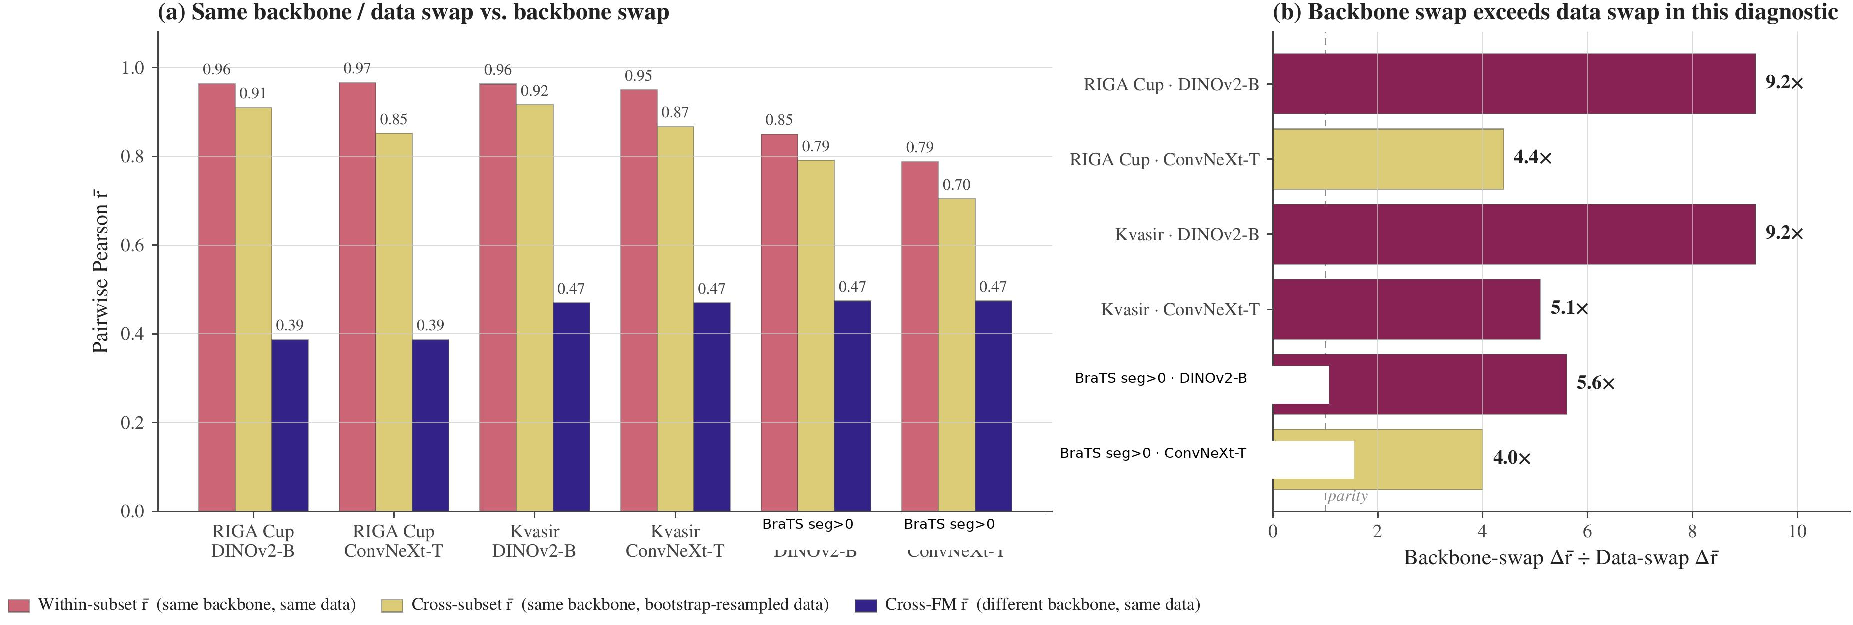
\includegraphics[width=\linewidth]{../figures/fig_phase3.pdf}
  \caption{\textbf{Same-backbone bootstrap-bagging diagnostic.} For each shown dataset/backbone pair, we compare (i) same-backbone/same-data cross-seed correlation, (ii) same-backbone/bootstrap-resampled-data correlation, and (iii) a cross-backbone reference from the corresponding diagnostic pool. The ratio panel reports $(r_{\mathrm{same\ data}}-r_{\mathrm{cross\ backbone}})/(r_{\mathrm{same\ data}}-r_{\mathrm{bootstrap\ data}})$, so values above one mean that changing backbone reduces correlation more than bootstrap-resampling the training data in this diagnostic. The BraTS label refers to the 2D foreground derivative (\texttt{seg>0}), not the official 3D BraTS WT challenge target. This figure is descriptive and does not identify a causal mechanism.}
  \label{fig:phase3}
\end{figure}

For each (FM, dataset) pair, four bootstrap replicates of the training set
(image-level on RIGA/Kvasir; subject-level on BraTS) are crossed with four
decoder seeds. Bootstrap data-swap reduces within-pool $\bar r$ by only
$0.05$--$0.12$, while backbone swap reduces it by $0.33$--$0.50$. This
supports the scoped claim that, in the frozen-feature protocol, resampling the
training cases does not provide the same decorrelation as changing encoder
family.

\section{Distribution-shift audit}
\label{app:distshift}

We evaluate one released cross-distribution robustness diagnostic for the
within--cross correlation gap using an 8-bundle RIGA pool and the frozen-feature
protocol from Section~\ref{sec:design}.

\textbf{RIGA leave-MESSIDOR-out (cross-vendor fundus).} RIGA+ \citep{riga_data} combines three imaging sources: \emph{BinRushed} (Bin Rushed Ophthalmic Center, Riyadh, Saudi Arabia), \emph{Magrabia} (Magrabi Eye Center, Riyadh, Saudi Arabia), and \emph{MESSIDOR} (French public corpus, different cameras and populations). We train the frozen-FM + $1{\times}1$ conv decoder on BinRushed+Magrabia (union) and evaluate on MESSIDOR ($454$ cases after local preprocessing/eligibility filtering from the 460-image MESSIDOR subset) as cross-vendor out-of-distribution. Per-case traces for this diagnostic are released under \texttt{results/\_merged/per\_case\_dice/riga\_cup\_ood\_messidor}. The released scorer uses a fixed 8-bundle $\times$ 4-seed pool without a functional-floor change between ID and OOD rows. Under that directly reproducible convention, the ID row has within/cross/gap $0.659/0.282/0.377$ and the MESSIDOR OOD row has $0.743/0.390/0.353$.

\textbf{Pool-level summary.} In this fixed-pool RIGA cross-vendor diagnostic, the within--cross gap changes by $-0.024$ and remains positive. Both within and cross correlations are higher on the MESSIDOR row, so this diagnostic should be read only as evidence that the gap survives one released cross-vendor stress test, not as evidence that distribution shift generally contracts dependence. Broader cross-scanner, cross-demographic, and longitudinal shifts remain out of scope.

\begin{table}[!htbp]
  \caption{\textbf{RIGA cross-vendor diagnostic under a fixed 8-bundle scorer.} This is not case-identical to Table~\ref{tab:main}. Within = same-FM different-seed $\cup$ same-family different-FM (DINOv2-B/S and ResNet-18/50); cross = different-family different-FM. The gap remains positive, but both within and cross correlations increase on MESSIDOR; no general distribution-shift conclusion is supported. Brackets are case-level bootstrap $95\%$ CIs ($B{=}500$). Source: \texttt{results/\_merged/diagnostics/distshift\_riga\_messidor.json}.}
  \label{tab:distshift}
  \centering\scriptsize
  \setlength{\tabcolsep}{3pt}
  \begin{tabularx}{\linewidth}{Yccc}
    \toprule
    Shift regime & Within-$\bar{r}$ & Cross-$\bar{r}$ & Gap \\
    \midrule
    ID reference (fixed 8-bundle pool) & $0.659$ [$0.603$, $0.715$] & $0.282$ [$0.197$, $0.369$] & $0.377$ [$0.301$, $0.463$] \\
    OOD MESSIDOR (fixed 8-bundle pool) & $0.743$ [$0.722$, $0.765$] & $0.390$ [$0.345$, $0.430$] & $0.353$ [$0.318$, $0.388$] \\
    \bottomrule
  \end{tabularx}
  \\[2pt]
  {\footnotesize This diagnostic uses a paired fixed 8-bundle RIGA pool and should not be read as a case-identical comparison to the Magrabia-source held-out primary RIGA rows in Table~\ref{tab:main}.}
\end{table}


\section{UNet-with-skip decoder replication}
\label{app:unet}

The paper's primary decoder is a $1{\times}1$ conv with $C{+}1$ trainable parameters for $C$ frozen channels (for example, 769 parameters for a 768-channel feature map), which is close to a linear probe on frozen features. Dense decoders with skip connections---nnU-Net, U-Net, SegFormer---are closer to deployed medical segmentation. We therefore ran a separate diagnostic in which the frozen backbone is unchanged but the head is replaced by a multi-scale UNet-style decoder over four encoder feature levels. This is a \emph{two-seed diagnostic grid} (seeds 42/43), not an inferential table with the same status as the four-seed primary pool; the reported correlation is the single seed-pair Pearson coefficient for each cell.

\textbf{Architecture.} For hierarchical CNNs (ConvNeXt-T, ResNet-50) the decoder uses the native feature pyramid as skip sources; for ViT-style encoders (DINOv2-B/S and BiomedCLIP ViT) it uses sampled intermediate token maps reassembled into a four-level pyramid. The released head first applies lateral $1{\times}1$ projections to a common decoder width, then runs a top-down bilinear-upsample path with three additive skip merges (deep $\to$ mid $\to$ shallow $\to$ shallowest), two conv-BN-ReLU blocks after each merge, a final conv-BN-ReLU after upsampling to the output grid, and a final $1{\times}1$ output conv. Training matches the frozen-feature recipe where possible: Adam lr $10^{-3}$, batch 16, 30 epochs, BCE, seeds $\{42,43\}$.

\begin{table}[!htbp]
  \caption{\textbf{Two-seed UNet-skip same-backbone diagnostic.} Each cell uses the two completed seeds 42/43 from the released UNet-skip trace tree; ``seed-pair $r$'' is therefore one Pearson coefficient, not a bootstrapped four-seed within-family estimate. Primary Table~\ref{tab:main} cross references are Kvasir 0.697, ACDC 0.639, RIGA Cup 0.361, and BraTS foreground 0.623.}
  \label{tab:unet}
  \centering\scriptsize
  \setlength{\tabcolsep}{3pt}
  \begin{tabular}{llcc}
    \toprule
    Task & Backbone & Mean Dice & Seed-pair $r$ \\
    \midrule
    Kvasir & DINOv2-B & 0.883 & 0.877 \\
    Kvasir & DINOv2-S & 0.866 & 0.919 \\
    Kvasir & BiomedCLIP & 0.806 & 0.926 \\
    Kvasir & ConvNeXt-T & 0.860 & 0.775 \\
    Kvasir & ResNet-50 & 0.816 & 0.774 \\
    \addlinespace
    ACDC LV & DINOv2-B & 0.864 & 0.979 \\
    ACDC LV & DINOv2-S & 0.863 & 0.970 \\
    ACDC LV & BiomedCLIP & 0.827 & 0.950 \\
    ACDC LV & ConvNeXt-T & 0.885 & 0.917 \\
    ACDC LV & ResNet-50 & 0.882 & 0.945 \\
    \addlinespace
    RIGA Cup & DINOv2-B & 0.902 & 0.967 \\
    RIGA Cup & DINOv2-S & 0.894 & 0.893 \\
    RIGA Cup & BiomedCLIP & 0.880 & 0.892 \\
    RIGA Cup & ConvNeXt-T & 0.895 & 0.970 \\
    RIGA Cup & ResNet-50 & 0.881 & 0.952 \\
    \addlinespace
    BraTS foreground & DINOv2-B & 0.877 & 0.936 \\
    BraTS foreground & DINOv2-S & 0.875 & 0.886 \\
    BraTS foreground & BiomedCLIP & 0.858 & 0.929 \\
    BraTS foreground & ConvNeXt-T & 0.895 & 0.938 \\
    BraTS foreground & ResNet-50 & 0.889 & 0.934 \\
    \bottomrule
  \end{tabular}
\end{table}

\textbf{Finding.} The UNet-skip head improves mean Dice substantially over several weak $1{\times}1$ probe cells, but it does not remove same-backbone co-failure: across the 20 evaluated cells, the seed-pair correlation remains $0.774$--$0.979$. On rows where the matched $1{\times}1$ seeds 42/43 are both available, UNet-skip usually lowers seed-pair $r$ modestly, but the effect is heterogeneous: Kvasir ResNet-50 drops $0.973{\to}0.774$, while RIGA Cup DINOv2-B is flat ($0.965{\to}0.967$) and RIGA Cup ResNet-50 increases ($0.908{\to}0.952$). The BraTS cells are consistent with the same boundary: DINOv2-B/S UNet-skip reaches mean Dice $0.875$--$0.877$, but seed-pair $r$ remains $0.886$--$0.936$. Thus the conclusion is narrower than a decoder-family claim: a stronger skip decoder can improve accuracy and sometimes reduce seed correlation, but under this frozen-backbone two-seed grid it does not make same-backbone pools resemble the cross-family references in Table~\ref{tab:main}. A full nnU-Net v2 $5$-fold audit on RIGA Cup is reported in Appendix~\ref{app:nnunet}.



\section{Fold-reslicing and nnU-Net complements}
\label{app:nnunet}

\textbf{Motivation.} nnU-Net \citep{isensee2021nnunet} is the de facto standard for medical image segmentation; its 5-fold cross-validation ensemble is a routinely-used uncertainty / robustness baseline. The full nnU-Net pipeline is \emph{self-configuring} (2D/3D selection, preprocessing, patch-based sampling, default geometric/intensity augmentation, cascaded network, post-processing). We keep two evidence surfaces separate: (i) the released frozen-feature fold-reslicing diagnostic, which tests split sensitivity with one decoder seed per fold and therefore cannot estimate within-fold versus cross-fold same-backbone pairs; and (ii) released task-level nnU-Net summary JSONs, which are full-pipeline complements but not case-identical contrasts to the primary FM rows.

\textbf{Released fold-reslicing design.} This diagnostic re-slices the frozen-feature cache into $5$ folds and reruns the 8-bundle pool $\{$DINOv2-B/S, BiomedCLIP, CLIP-L, ConvNeXt-T, EfficientNet-B0, ResNet-50/18$\}$ on ACDC LV and RIGA Cup, single seed per fold cell. Because the released artifact contains one seed per fold, this diagnostic reports per-fold cross-bundle $\bar r$ and pool-mean Dice, not a 20-decoder fixed-backbone within/cross estimator. The released artifact provides the corresponding fold-reslicing summary and scorer.

\begin{table}[!htbp]
  \caption{\textbf{Fold-reslicing cross-bundle stability, one seed/fold.} 8 bundles $\times$ 5 folds; single seed per fold cell. Cross-bundle $\bar r$ is the Pearson correlation averaged over the 28 bundle pairs on the held-out fold. This table cannot support within-fold versus cross-fold same-backbone claims.}
  \label{tab:m15-fold}
  \centering\small
  \begin{tabular}{lrrrrrr}
    \toprule
    Task & fold 0 & fold 1 & fold 2 & fold 3 & fold 4 & mean$\,\pm\,$std \\
    \midrule
    ACDC LV  & $0.580$ & $0.548$ & $0.583$ & $0.558$ & $0.558$ & $0.565 \pm 0.015$ \\
    RIGA Cup & $0.359$ & $0.317$ & $0.325$ & $0.315$ & $0.261$ & $0.315 \pm 0.035$ \\
    \bottomrule
  \end{tabular}
\end{table}

\textbf{Finding.} Train/test split sensitivity is small in this fold-reslicing check: cross-fold pool-mean Dice is stable (ACDC $0.502 \pm 0.022$; Cup $0.610 \pm 0.012$), and per-fold cross-bundle $\bar r$ is stable across folds (ACDC $0.565 \pm 0.015$; Cup $0.315 \pm 0.035$). This supports only the narrower statement that the cross-bundle diagnostic is not dominated by one particular 5-fold re-slicing. It does \emph{not} support a claim about within-fold vs cross-fold same-backbone decorrelation, because those pair types require multiple decoder seeds per fold that are not present in the released traces.

\paragraph{Full nnU-Net v2 complement.} To complement the frozen-feature proxy above and answer whether nnU-Net's full self-configuring pipeline decorrelates the pool more, we trained the full nnU-Net v2 2D U-Net on RIGA Cup with a $520/224$ split, using the generated v2 2D \texttt{nnUNetPlans} configuration after \texttt{nnUNetv2\_plan\_and\_preprocess} (self-configured preprocessing and architecture, official default augmentation/loss schedule, $250$ iterations per epoch). This split differs from the Magrabia-source held-out FM row and is therefore a task-level complement. We train two seeds per fold via custom \texttt{nnUNetTrainerSeed13\_100epochs} and \texttt{nnUNetTrainerSeed37\_100epochs} subclasses that pre-seed \texttt{random}, \texttt{np.random}, \texttt{torch}, and \texttt{cuda} before any nnU-Net sampler touches the RNG; each is trained for $100$ nnU-Net-epochs ($25{,}000$ iterations on two A100s in parallel), then all $5\times 2{=}10$ models predict on the held-out $224$-image test set via \texttt{nnUNetv2\_predict} and per-case Dice is computed against the held-out labels staged in \texttt{labelsTr}. The local nnU-Net export used a split-index file to enumerate held-out IDs; the artifact bundle releases the summary arrays/JSONs for this complement but not that local split manifest.

Across all $10$ models the mean Dice is $0.949\pm 0.001$ (exceeding any of our frozen-feature FM$+1{\times}1$-conv combinations on RIGA Cup). The pairwise per-case Dice $\bar{r}$ is $0.972$ within-fold over the $5$ same-fold different-seed pairs and $0.925$ cross-fold over the $40$ different-fold any-seed pairs, with $\Delta_{\mathrm{within-cross}}{=}0.047$ and a case-level bootstrap $95\%$ CI of $[0.030, 0.069]$ that excludes zero. Full nnU-Net v2 is structurally a same-architecture, different-training-data ensemble on one 2D PlainConvUNet, so it is not comparable in kind to the primary frozen-FM cross-family reference, which swaps encoder bundles. The scoped conclusion is therefore: \emph{within this task-level same-architecture nnU-Net complement, fold identity leaves a small but positive correlation gap}; we do not claim nnU-Net substitutes for or surpasses backbone-family diversification. The $100$-epoch budget, single-task coverage, and 2D-only scope are closed in Appendix~\ref{app:w1-scope} (1000-epoch retrain on the same RIGA Cup setup; 3D fullres nnU-Net on ACDC; higher-resolution/Dice+BCE/aug frozen-FM replication).

\paragraph{Data-swap comparison caveat.} Appendix~\ref{sec:samebb} reports bootstrap-bagging within-pool decorrelation with four decoder seeds per bootstrap replicate. The fold-reslicing row instead reports single-seed cross-bundle correlations across held-out folds. These diagnostics both stress training data/split sensitivity, but they are not dose-matched estimators and are not combined into a causal ranking.


\section{Segmentation-recipe and nnU-Net scope audit}
\label{app:w1-scope}

Our main protocol uses $224{\times}224$ 2D inputs, frozen backbone, $1{\times}1$-conv decoder, BCE loss, no augmentation, and 30-epoch head training. Routine medical-imaging pipelines often run with compound Dice$+$CE loss, geometric augmentation, 3D input, and full-length ($1000$-epoch) training, so we test whether the within/cross correlation structure we report is specific to the simplified protocol. We close these axes as task-level complements; the RIGA nnU-Net rows use a different 520/224 split rather than the Magrabia-source held-out FM split, so they should not be read as case-identical contrasts.

\paragraph{Dimensionality axis: 3D fullres nnU-Net at 1000 epochs on ACDC.}
Training nnU-Net v2 in its self-configuring \texttt{3d\_fullres} setting on ACDC with a seed-42 $105{/}45$-patient split (210 training, 90 test volumes) using \texttt{nnUNetTrainerSeed\{13,37\}\_1000epochs} (seed injected in \texttt{on\_train\_start} before sampler initialisation) gives 10 fully-trained 3D models across 5 folds. \texttt{nnUNetv2\_predict} on all 90 held-out volumes yields per-case Dice on mean foreground and per class. Across 10 models the mean Dice is $0.920 \pm 0.001$, within the range reported for strong nnU-Net baselines on ACDC. On per-case mean Dice the within-fold (5 pairs) vs cross-fold (40 pairs) gap is $\Delta{=}0.043$ [0.021, 0.085] with within $\bar r{=}0.978$ and cross $\bar r{=}0.935$; per class, $\Delta_{\mathrm{RV}}{=}0.041$ [0.011, 0.110], $\Delta_{\mathrm{Myo}}{=}0.029$ [0.017, 0.046], $\Delta_{\mathrm{LV}}{=}0.067$ [0.033, 0.098]. The artifact bundle releases the aggregate summary for this 150-patient complement but not the exact split manifest; the released public ACDC converter targets patients 001--100 for the primary 2D row. We therefore treat this 3D row as a task-level scope summary rather than a from-bundle training recipe. In this ACDC nnU-Net complement, the 2D$\to$3D fullres shift changes the small fold-gap regime by less than $0.01$ relative to the 2D 100-epoch baseline ($\Delta{=}0.047$ in Appendix~\ref{app:nnunet}).

\paragraph{Loss / augmentation axis: RIGA Cup frozen-FM at encoder-native $224{\times}224$.}
We retrain the seven-bundle RIGA Cup subset (DINOv2-B/S, CLIP ViT-L/14, ConvNeXt-T, EfficientNet-B0, ResNet-50/18) with four seeds each under a more standard segmentation loss/augmentation recipe: encoder-native input size $224{\times}224$, composite soft Dice$+$BCE loss, paired random horizontal flip and rotation $\pm 15^\circ$, for 30 epochs. The frozen encoder wrappers use $224{\times}224$ inputs; we therefore treat this as a loss/augmentation test, not a resolution test. All other factors (frozen backbone, $1{\times}1$-conv segmentation head, Adam $10^{-3}$) match the main protocol.
Per-FM mean Dice ranges from $0.526$ (ResNet-18) to $0.758$ (DINOv2-B). Under the same symmetric estimator used for the main table, within-family $\bar r$ is $0.903$ (58 within pairs, including same-FM seed pairs and DINOv2-B$\times$S), cross-FM $\bar r$ is $0.556$ (320 cross pairs), and the within/cross gap is $\Delta{=}0.347$ [0.275, 0.428]. The gap is smaller than the main RIGA Cup interval ($0.473$ [0.395, 0.556]) but remains positive; loss/augmentation changes do not remove the gap.

\paragraph{Training-length axis: full nnU-Net v2 at the 1000-epoch default on RIGA Cup.}
We retrain the 10-model RIGA Cup 2D nnU-Net pool from Appendix~\ref{app:nnunet} at the nnU-Net v2 default 1000 epochs, using the same seeded trainer pattern (\texttt{nnUNetTrainerSeed\{13,37\}\_1000epochs}) on the same $520/224$ split with identical dataset/plan files. Mean Dice across the 10 models is $0.946 \pm 0.0004$ (vs $0.949 \pm 0.001$ at 100 epochs). Within-fold $\bar r{=}0.983$ (5 pairs), cross-fold $\bar r{=}0.949$ (40 pairs), and $\Delta{=}0.034$ [0.021, 0.058]. Relative to the 100-epoch run both estimators tighten slightly (within $0.972{\to}0.983$; cross $0.925{\to}0.949$) and the within/cross gap contracts from $0.047$ to $0.034$; measured predictions are more correlated under longer training, and the gap does not disappear. Ten-fold longer training therefore does not change the replicability structure of nnU-Net on this task-level complement; it is not a case-identical comparison to the Magrabia-source held-out FM row.

\paragraph{Synthesis.}
Across these scope analyses, the frozen-FM loss/augmentation row remains in the same large-gap regime as the RIGA Cup main row, while the same-architecture nnU-Net fold axis remains in the small-gap regime ($\Delta \approx 0.04$). Because the nnU-Net RIGA rows use a different split, the synthesis is a task-level scope check rather than a paired case-identical comparison. These rows do not support a simpler explanation that the main-table pattern is solely an artifact of BCE loss, no augmentation, short training, or the tested full-pipeline nnU-Net complements.

\begin{table}[!htbp]
  \caption{\textbf{Scope audit across recipe and nnU-Net complements.} Rows are not all case-identical and should not be compared as a controlled ablation. The table asks whether selected recipe changes remove the qualitative gap. The frozen-reference row uses the same seven candidate FMs as the Dice+BCE+augmentation row before the primary functional-floor exclusion; the primary filtered RIGA Cup row is Table~\ref{tab:main}. The RIGA nnU-Net rows use a different 520/224 split and are not case-identical comparisons to the Magrabia-source held-out FM row.}
  \label{tab:w1-scope}
  \centering\scriptsize
  \setlength{\tabcolsep}{2.5pt}
  \begin{tabularx}{\linewidth}{p{0.16\linewidth}Yp{0.12\linewidth}cccc}
    \toprule
    Axis & Protocol & Task & Within & Cross & $\Delta$ & 95\% CI \\
    \midrule
    Frozen reference & 7-bundle candidate set, $224$, BCE, no aug, 30 epochs & RIGA Cup & $0.798$ & $0.266$ & $0.532$ & $[0.456, 0.614]$ \\
    Loss / aug & 7-bundle frozen, $224$, Dice+BCE, aug, 30 epochs & RIGA Cup & $0.903$ & $0.556$ & $0.347$ & $[0.275, 0.428]$ \\
    \midrule
    Baseline (App.~\ref{app:nnunet}) & nnU-Net 2D, $100$ epochs & RIGA Cup & $0.972$ & $0.925$ & $0.047$ & $[0.030, 0.069]$ \\
    Training length & nnU-Net 2D, $1000$ epochs & RIGA Cup & $0.983$ & $0.949$ & $0.034$ & $[0.021, 0.058]$ \\
    \midrule
    Dimensionality & nnU-Net 3D fullres, $1000$ep & ACDC (mean) & $0.978$ & $0.935$ & $0.043$ & $[0.021, 0.085]$ \\
    & \hspace{1em}per-class RV & & $0.967$ & $0.927$ & $0.041$ & $[0.011, 0.110]$ \\
    & \hspace{1em}per-class Myo & & $0.987$ & $0.957$ & $0.029$ & $[0.017, 0.046]$ \\
    & \hspace{1em}per-class LV & & $0.978$ & $0.911$ & $0.067$ & $[0.033, 0.098]$ \\
    \bottomrule
  \end{tabularx}
\end{table}


\section{Held-out multi-task stress test}
\label{app:heldout}

\textbf{Protocol.} In addition to the four primary benchmark datasets (five task rows: Cup, Disc, ACDC, Kvasir, BraTS foreground), we evaluate five \emph{held-out} tasks covering additional imaging domains: MSD Hippocampus \citep{msd2022} (T1 MRI, native 3-class mask \{background, anterior, posterior\} binarized to \{background, any-hippocampus\}), ISIC-2018 Task 1 Lesion Boundary \citep{isic2018} (dermoscopy, 2D RGB, $N{=}80$ test cases held out from a 400-image random subset of the 2{,}594-image training release), MSD Heart (T2 MRI cardiac), MSD Prostate (T2 MRI prostate), and MSD Spleen (CT portal). This held-out stress test uses the same 11 generic encoder bundles and four decoder seeds as the primary source pool where possible, with the same 1$\times$1-conv decoder, no per-task hyperparameter tuning, and no model substitution. These are task-specific 2D binary derivatives, not official challenge-test evaluations. The Dice${\geq}0.30$ functional floor is applied uniformly, and the released aggregate summary records 220/220 expected per-seed traces.

\begin{table}[!htbp]
  \caption{\textbf{Held-out aggregate stress test} (11 generic encoder bundles $\times$ 4 decoder seeds; point estimates only, no case-bootstrap CIs). Hippocampus and ISIC-2018 are direction-positive, Prostate is positive but has only six test cases, Spleen is essentially near-zero despite passing the Dice floor, and Heart has no functional bundle at the Dice${\geq}0.30$ floor. Tiny-$N$ and floor-failure rows are scope boundaries and do not support the primary claim.}
  \label{tab:heldout}
  \centering\scriptsize
  \setlength{\tabcolsep}{3pt}
  \begin{tabular*}{\linewidth}{@{\extracolsep{\fill}}lcccccc}
    \toprule
    Task & $N$ & Func./avail. & Within & Cross & $\Delta$ & $M_{\text{eff}}$ \\
    \midrule
    \multicolumn{7}{l}{\emph{Direction-positive point estimates with enough support to read qualitatively}} \\
    MSD Hippocampus   & 52  & 11/11 & 0.909 & 0.419 & \textbf{0.491}$^{\S}$ & 3.94 \\
    ISIC-2018$^{\ddagger}$ & 80 & 11/11 & 0.918 & 0.511 & \textbf{0.406}$^{\S}$ & 2.72 \\
    \midrule
    \multicolumn{7}{l}{\emph{Scope-limit rows: tiny held-out support or non-functional pool}} \\
    MSD Prostate & 6 & 5/11 & 0.788 & 0.642 & 0.146$^{\S}$ & 1.23 \\
    MSD Spleen   & 8 & 11/11 & 0.983 & 0.979 & 0.003$^{\S}$ & 1.02 \\
    MSD Heart    & 4 & 0/11 & ---$^{*}$ & ---$^{*}$ & ---$^{*}$ & --- \\
    \bottomrule
  \end{tabular*}
  \\[2pt]
  {\footnotesize $^{*}$No bundle passes the Dice${\geq}0.30$ floor on the four-case Heart derivative, so no within/cross gap is interpretable. $^{\S}$Values are point estimates from \texttt{results/\_merged/diagnostics/heldout\_11fm\_summary.json}; case-level CIs are not computed for this aggregate diagnostic, and the MSD Prostate/Spleen rows have too few held-out cases to support a primary claim. $^{\ddagger}$ISIC-2018 uses a single random $N{=}400$-image subset of the 2{,}594-image ISIC-2018 training release with $N{=}80$ test cases under the seed-42 80/20 split; we do not report an independent redraw and we do not use the official ISIC test server in this study.}
\end{table}

\textbf{Interpretation.} The 11-bundle held-out protocol yields three classes of outcome: (i)~ISIC-2018 and Hippocampus both show direction-positive gaps under the same broad estimator family as the primary audit, but without case-bootstrap CIs and with smaller held-out support than the primary rows. (ii)~Prostate and Spleen illustrate why held-out diagnostics are scope boundaries rather than headline evidence: Prostate is direction-positive but has only six test cases, while Spleen passes the floor yet has a near-zero gap and $M_{\text{eff}}\approx1$ because the members fail together. (iii)~Heart does not yield a functional pool under the frozen-feature 2D derivative. Thus the held-out stress test is compatible with transfer to some external rows, but it also records where the protocol is too weak or too saturated to audit same-bundle dependence.

\textbf{Operational 8-bundle held-out probes.} The following recovery, pool-size, abstention, and pool-selection diagnostics use an 8-bundle held-out candidate set stored under \texttt{results/\_merged/diagnostics/held\_out/}. They are retained as operational-method sensitivities, not as the provenance for Table~\ref{tab:heldout} above.

\textbf{CLIP/BiomedCLIP normalization robustness.} Uniform ImageNet normalization can be a potential artifact for BiomedCLIP and CLIP-L because both have their own normalization statistics. We therefore evaluated those two FMs on Hippocampus and ISIC-2018 with the correct CLIP normalization. The released \texttt{summary\_clipfix.json} reports BiomedCLIP mean Dice $0.840$ (Hippocampus) / $0.908$ (ISIC-2018), while CLIP-L remains below the functional floor on Hippocampus (mean Dice ${<}10^{-10}$) and reaches $0.106$ on ISIC-2018, still below the $0.30$ floor. Relative to \texttt{summary\_5tasks.json}, the aggregate $\Delta$ changed by $0.002$ (Hippocampus $0.731{\to}0.729$) and $0.003$ (ISIC-2018 $0.552{\to}0.555$). In this held-out diagnostic, correcting CLIP/BiomedCLIP normalization does not materially change the Hippocampus/ISIC point estimates.

\textbf{Held-out recovery-rate sensitivity.} To complement the primary-task $\Delta_{\text{rec}}{=}+0.29$ (Cup) / $+0.26$ (ACDC) grand means, we computed an exploratory held-out recovery gap at $\tau{=}0.85$ on the single ISIC-2018 subset: $\Delta_{\text{rec}}{=}+0.269$~[$+0.212$,$+0.331$] under a case-resampling calculation saved as \texttt{recovery\_CI.json}. This supports the direction of the operational gap on one dermoscopy subset, but it is not a deployment-calibrated guarantee and does not resolve the held-out estimator-dependence above. Hippocampus at $\tau{=}0.85$ is recovery-saturated and gives $\Delta_{\text{rec}}{=}-0.01$~[$-0.03$, $+0.00$] (diverse and mono both near-zero recovery because only 2/7 functional bundles individually pass Dice${\geq}0.85$). Lower thresholds are not evaluated here.

\textbf{Pool-size sweep on held-out tasks.} How does diverse-vs-same-bundle conditional recovery scale with $M$? For $M{\in}\{2,3,4,5,6\}$ on the two functional held-out tasks (Table~\ref{tab:pool-size-sweep}), diverse pools beat same-bundle seed pools at every $M{\geq}3$ on the single ISIC-2018 subset ($\Delta_{\text{rec}}{=}0.27$--$0.46$), while Hippocampus at the paper's $\tau{=}0.85$ threshold is recovery-rate-saturated (all pools ${<}0.11$) because only 2 of 7 functional bundles reach Dice${\geq}0.85$ individually. These held-out operational analyses are exploratory: ISIC provides one supportive dermoscopy subset, Hippocampus is threshold-saturated at $\tau{=}0.85$, and the $M{=}5,6$ same-bundle rows are proxy constructions using the available four seeds rather than true larger same-bundle pools. Released aggregate data: \texttt{results/\_merged/diagnostics/held\_out/pool\_size\_sweep.json}.

\begin{table}[!htbp]
  \caption{\textbf{Exploratory held-out pool-size sweep.} Conditional recovery rate $P[\text{ens pass}\mid\text{any fail}]$ at $\tau{=}0.85$ vs pool size $M$. $M{=}2$ recovery is a definition artifact under the strict-majority rule, and $M{=}5,6$ same-bundle values are four-seed proxies. This table is not a deployable pool-size recommendation.}
  \label{tab:pool-size-sweep}
  \centering\small
  \begin{tabular}{c|ccc|ccc}
    \toprule
    & \multicolumn{3}{c|}{Hippocampus} & \multicolumn{3}{c}{ISIC-2018} \\
    $M$ & mono & diverse & $\Delta$ & mono & diverse & $\Delta$ \\
    \midrule
    2$^{\dagger}$ & 0.000 & 0.000 & $+0.00$ & 0.000 & 0.000 & $+0.00$ \\
    3 & 0.069 & 0.107 & $+0.04$ & 0.111 & 0.498 & $+0.39$ \\
    4 & 0.052 & 0.039 & $-0.01$ & 0.091 & 0.359 & $+0.27$ \\
    5$^{\ddagger}$ & 0.052 & 0.078 & $+0.03$ & 0.091 & 0.553 & $+0.46$ \\
    6$^{\ddagger}$ & 0.052 & 0.027 & $-0.03$ & 0.091 & 0.454 & $+0.36$ \\
    \bottomrule
  \end{tabular}
  \\[2pt]
  {\footnotesize $^{\dagger}$$M{=}2$ is a definition artifact under the strict-majority (${>}M/2$) rule conditioned on any-fail: recovery is zero by construction whenever $M{=}2$, regardless of pool composition. We include the row for completeness. $^{\ddagger}$At $M{=}5,6$ the same-bundle entries are computed on the $\min(M,S){=}4$ available seeds per FM, so they do not represent true $M{=}5,6$ same-bundle pools; the diverse entries do use legitimate $M{=}5,6$ distinct-family compositions.}
\end{table}

\textbf{Calibration-tuned disagreement-based abstention (an exploratory alternative lever, not a conformal guarantee).} A natural operational question is whether standard abstention-based uncertainty gating closes the same-bundle gap with modest additional computation. We calibrate a per-task disagreement-score threshold on 20 cases (inter-member Dice standard deviation as score; grid-search the quantile $q$ to meet a target case-risk $\alpha{=}0.1$ on calibration; apply the selected threshold to the remaining test cases). \emph{This is a tuned heuristic, not split-conformal prediction} \citep{angelopoulos2021gentle}: we use a grid search over $q$ that terminates on the first calibration risk meeting $\alpha$ and use inter-member variance rather than a proper conformity score, so no finite-sample risk guarantee holds. The pool is also chosen per-task on the whole task mean Dice (family-representative highest-Dice FMs), so the diverse-pool selection step leaks task labels---this biases the comparison toward diverse pools. We report it as a sensitivity. On ISIC-2018 at matched abstention $\approx 0.74$, diverse pools reach test-risk $0.129{\pm}0.027$ vs.\ same-bundle grand mean $0.174{\pm}0.209$ (\texttt{conformal\_vs\_meff.json}). The \emph{point estimate} is $\sim 25\%$ lower for diverse, but the same-bundle grand-mean SD ($0.21$) is $\sim 8{\times}$ the diverse SD ($0.027$); the per-FM same-bundle risk means span $0.000$--$0.616$ across the seven functional FMs, so the grand-mean comparison is highly composition-sensitive and we do not claim a tight ranking. Hippocampus cannot hit $\alpha{=}0.1$ for either pool, giving residual risk $0.694$ (diverse) vs.\ $0.665$ (same-bundle grand mean) ($\Delta{=}+0.03$, with same-bundle SD $0.28$, indistinguishable). A label-free conformal procedure with a proper conformity score is not evaluated here. Released aggregate data: \texttt{results/\_merged/diagnostics/held\_out/conformal\_vs\_meff.json}.

\textbf{Calibration-set pool-selection probe on held-out tasks.} We operationalise a small calibration exercise: given only a 20-case calibration set on a held-out task, can a rule pick a 4-of-8 FM pool from the same secondary held-out candidate set that beats random? We evaluate five rules---(R1) random, (R2) top-4 by mean Dice on calibration, (R3) max-$M_{\text{eff}}$, (R4) quality-gated max-$M_{\text{eff}}$ (Dice${\geq}0.30$ floor then max-$M_{\text{eff}}$ among qualifying), (R5) diverse-by-architecture (2 best-Dice ViT $+$ 2 best-Dice CNN; reported as an exploratory hand-crafted baseline, not a general proposal)---and report conditional recovery rate $P[\text{ens pass}\mid\text{any fail}]$ at $\tau{=}0.85$ on the remaining held-out cases, averaged over 100 calibration-set bootstraps (Table~\ref{tab:pool-challenge}). All rule selectors and the recovery estimator use seed-42 per-case Dice (not seed-averaged), matching a one-model-per-FM pool construction. Hippocampus has lower effective recovery support than ISIC at $\tau{=}0.85$, so its recovery numbers are exploratory. In this diagnostic, simple top-4-by-Dice has the highest mean on both tasks (Hippocampus 0.161 vs.\ 0.043 random; ISIC-2018 0.581 vs.\ 0.378 random), while max-$M_{\text{eff}}$ alone is worse than random (0.011 / 0.327). This supports the narrower point that $M_{\text{eff}}$ is a dependence readout rather than a standalone operational objective; it is not a validated clinical pool-selection rule. Released aggregate data: \texttt{results/\_merged/diagnostics/held\_out/pool\_selection\_challenge.json}.

\begin{table}[!htbp]
  \caption{\textbf{Exploratory pool-selection probe.} Conditional recovery rate at $\tau{=}0.85$ (mean $\pm$ SD over 100 calibration bootstraps, 20 cases each, using seed-42 traces). Selection uses calibration labels. This probes whether $M_{\text{eff}}$ alone is a poor objective; it is not a validated clinical selection rule.}
  \label{tab:pool-challenge}
  \centering\small
  \begin{tabular}{lcc}
    \toprule
    Rule & Hippocampus & ISIC-2018 \\
    \midrule
    (R1) Random 4-of-8                        & 0.043$\,\pm\,$0.050 & 0.378$\,\pm\,$0.125 \\
    (R2) Top-4 by calibration Dice            & \textbf{0.161}$\,\pm\,$0.017 & \textbf{0.581}$\,\pm\,$0.030 \\
    (R3) Max $M_{\text{eff}}$                 & 0.011$\,\pm\,$0.011 & 0.327$\,\pm\,$0.100 \\
    (R4) Quality-gated max $M_{\text{eff}}$   & 0.016$\,\pm\,$0.014 & 0.381$\,\pm\,$0.112 \\
    (R5) Diverse-by-arch (2 ViT $+$ 2 CNN)    & 0.096$\,\pm\,$0.017 & 0.445$\,\pm\,$0.036 \\
    \bottomrule
  \end{tabular}
\end{table}

\textbf{Held-out estimator note.} Split-stability and alternate-estimator numerical summaries whose exact aggregate files are not included in the supplementary artifact are omitted from the numeric evidence. This section therefore relies on the released 11-bundle held-out aggregate and the released operational JSONs listed above.

\textbf{ISIC-2018 single-subset note.} The ISIC-2018 row above is a single random $N{=}400$-image subset of the ISIC-2018 Task 1 training release with $N{=}80$ held-out test cases under a seed-42 80/20 split. We do not report an independent replication of this subset; a fully random redraw of the subset or use of the official ISIC evaluation server would be a natural next step but is out of scope for this paper.

\section{MC dropout diagnostic scope}
\label{app:mcdrop}

A separate MC-dropout probe suggested lower any-draw correlations, but its traces are not included in the supplementary artifact and its scorer differs from the released averaged-readout diagnostic. We therefore do not tabulate it or use it as evidence. The released MC-dropout diagnostic is Appendix~\ref{app:m22}: under the deterministic-vs-MC-averaged readout, $p{=}0.1$--$0.4$ reduces within-FM $\bar r$ only from roughly $0.97$--$0.99$ to $0.95$--$0.89$, so MC dropout is a weak within-family lever in this diagnostic and does not approach the tested backbone-family swap.



\section{Full fine-tuning scope}
\label{app:ftsweep}

RIGA Cup full fine-tuning epoch-sweep traces and aggregate summaries are not
included in the supplementary artifact. We therefore do not tabulate those values or use them as
numerical evidence. The released adaptation evidence is limited to
released traces and summaries named elsewhere in the appendix, including a small
set of ACDC DINOv2-B full-fine-tuning provenance traces but not the RIGA
epoch-sweep matrix; full-fine-tuning numbers not backed by released paths should
be read only as exploratory mechanism notes and not as support for the paper's
claims.

\section{Same-backbone and scope diagnostic index}
\label{app:lever}

\begin{table}[!htbp]
  \caption{\textbf{Qualitative index of same-backbone and scope diagnostics}. Rows are heterogeneous and not CI-comparable; the table is a navigation aid, not an ordered causal hierarchy. The RIGA-oriented map is anchored on the DINOv2-B 4-seed baseline ($\bar{r}{\approx}0.96$) unless marked. LoRA, full-fine-tuning epoch-sweep, and ViT random-init probes whose traces are not distributed are omitted.}
  \label{tab:lever}
  \centering\scriptsize
  \setlength{\tabcolsep}{2.5pt}
  \begin{tabularx}{\linewidth}{p{0.30\linewidth}c p{0.16\linewidth}Y}
    \toprule
    Diagnostic & Readout & Approx. change from stated baseline & Evidence \\
    \midrule
    Mono baseline (same FM, 4 seeds)                       & $0.96$                           & $0.00$                       & RIGA diagnostic baseline \\
    UNet-skip decoder (5 backbones, 4 tasks)               & $0.774$--$0.979$                 & heterogeneous                & Appx.~\ref{app:unet}, Tab.~\ref{tab:unet} \\
    Fold-reslicing cross-bundle check                      & $0.315$--$0.565$                 & split-stable                 & Appx.~\ref{app:nnunet}; released summary \\
    MC dropout $p{=}0.1$--$0.4$                            & $0.89$--$0.95$                   & $-0.02$ to $-0.10$           & Appx.~\ref{app:m22} \\
    Same-backbone bootstrap-bagging                        & $0.85$--$0.92$                   & $-0.05$ to $-0.12$           & Fig.~\ref{fig:phase3} \\
    RIGA cross-vendor shift                                & OOD w/c $0.743/0.390$             & gap $0.353$; $\Delta_{\mathrm{gap}}{-}0.024$ & Appx.~\ref{app:distshift} \\
    Decoder capacity sweep                                 & $\sim 0.69$                      & $\sim -0.27$                 & Appx.~\ref{app:m3} \\
    \midrule
    \textbf{Cross-family pretrained 8-bundle pool}         & $\mathbf{0.38}$~[$0.29$,~$0.46$] & $\mathbf{-0.58}$             & RIGA mechanism diagnostic \\
    \bottomrule
  \end{tabularx}
\end{table}



\section{Leave-one-family-out scope}
\label{app:lofo}

Leave-one-family-out summaries were used as exploratory robustness checks, but the
exact aggregate source is not included in the supplementary artifact. We therefore omit the
numeric table from the released evidence record. The primary
robustness check for the primary rows is the released
\texttt{diagnostics/audit\_sensitivity.json}, which includes leave-one-task and
leave-one-FM summaries under the same scorer path.

\section{Joint-failure lift at support limits}
\label{app:lift-ceiling}
Joint-failure lift $L{=}P_{\text{empirical joint}}/\prod_m P_{\text{marginal}}$ is unstable when marginal fail rates are near $0$ or near $1$. When $P_{\text{marginal}}\approx 0.3$, independence-implied joint $\approx 0.01$; small sampling variation in the empirical joint produces large lift ratios. Representative near-ceiling cells:
\begin{table}[!htbp]
  \caption{\textbf{Support-limit examples for joint-failure lift.} Extreme lifts are shown to explain instability, not to support a headline claim. Lifts $\ge 50\times$ are descriptive (support-limited, wide noise envelope) and are \emph{not} paper-headline statistics.}
  \label{tab:lift-ceiling}
  \centering\small
  \begin{tabular}{llrrr}
    \toprule
    Task / Pool & $\tau$ & Indep. joint & Empirical joint & Lift \\
    \midrule
    RIGA Cup mono BiomedCLIP  & 0.85 & 0.0010 & 0.125 & $123.2\times$ \\
    RIGA Cup mono DINOv2-B    & 0.85 & 0.0047 & 0.183 & $38.8\times$ \\
    RIGA Cup diverse 4-bundle & 0.85 & 0.0160 & 0.098 & $6.1\times$ \\
    ACDC LV mono DINOv2-B     & 0.70 & 0.0002 & 0.038 & $189\times$ \\
    ACDC LV diverse 4-bundle  & 0.85 & 0.135  & 0.378 & $2.8\times$ \\
    \bottomrule
  \end{tabular}
\end{table}
Only the ACDC $2.8\times$ row is adequately supported by the $N\cdot\mathbb{E}[\mathrm{AF}_{\mathrm{ind}}]\geq5$ rule. The RIGA Cup $6.1\times$ and $38.8\times$ rows are support-limited, and the $123.2\times$ and $189\times$ rows are extreme sparse-tail diagnostics.


\section{3D segmentation-architecture pilot}
\label{app:3dfm}
This section provides scope context only. Its per-case outputs and scorer version are not included in the supplementary artifact, so the pilot is not used as primary evidence for Table~\ref{tab:main}, the abstract, or the released artifact claims. It motivates why we avoid generalizing the frozen 2D FM-pool result to 3D segmentation-architecture pools.

We assembled a 3D segmentation-architecture pool for BraTS 2024 3D volumes (271 subjects, 216/55 train/test, seed 42) using three architectures in the implementation path: SegResNet (optionally initialised from the MONAI BraTS bundle), DynUNet (random-init), and UNETR (random-init). SwinUNETR random-init pilot cells were included initially but dropped after degenerate predictions across all seeds. For each retained (architecture, seed $\in\{42,43,44,45\}$) cell, the pilot trained the full MONAI segmentation model for 100 epochs with Adam $10^{-3}$ and BCE loss; UNETR-style models used sliding-window inference where required by memory. Reported at three filter modes:

\begin{table}[!htbp]
  \caption{\textbf{3D pilot for scope context only.} Per-case outputs and scorer version are not included in the supplementary artifact; this table is excluded from the abstract and main-result evidence. Three functional-filter modes are applied uniformly in the pilot. Strict filter (Dice $\geq 0.50$) retains only SegResNet pretrained and DynUNet random-init and yields $\Delta{=}0.045$, substantially below the 2D BraTS foreground $\Delta{=}0.315$.}
  \label{tab:3dfm}
  \centering\scriptsize
  \setlength{\tabcolsep}{3pt}
  \begin{tabularx}{\linewidth}{Ycccc}
    \toprule
    Filter & FMs retained & Within & Cross & $\Delta$ [95\% CI] \\
    \midrule
    Mixed (all cells)              & 3 (12 cells) & 0.772 & 0.595 & 0.177 [0.117, 0.248] \\
    Dice $\geq 0.30$                & 3 (12 cells, drop UNETR seed 43 degenerate) & 0.919 & 0.703 & 0.216 [0.134, 0.271] \\
    Dice $\geq 0.50$ (strict functional) & 2 (SegResNet pretrained, DynUNet random) & 0.916 & 0.871 & \textbf{0.045} [0.015, 0.112] \\
    \addlinespace
    Random-init only (DynUNet + UNETR) & 2 random-init & 0.724 & 0.479 & 0.245 [0.155, 0.351] \\
    \bottomrule
  \end{tabularx}
\end{table}

\textbf{Interpretation.} Within the strict functional regime (only converged pretrained + converged random-init CNN-style 3D architectures), the 3D segmentation-architecture pilot shows $\Delta{=}0.045$---substantially below the 2D BraTS foreground $\Delta{=}0.315$. We treat this only as a scope warning: the 2D frozen-feature same-bundle dependence claim should not be extended to 3D segmentation-architecture pools without a released, case-identical 3D benchmark. Random-init 3D architectures cross-correlate \emph{more} than pretrained 3D architectures (within random $0.724$ vs cross-architecture random $0.479$, $\Delta{=}0.245$), so architecture-family effects again appear large in this pilot. The degenerate SwinUNETR pilot cells limit architecture coverage in the 3D pilot; expanded 3D foundation-model evaluation (Models Genesis, Vista3D, Triad-MRI) is not evaluated here.

\section{Matched-recipe adaptation scope}
\label{app:matched-recipe}
\label{app:matched-recipe-acdc}

Matched-recipe adaptation factorials require source prediction caches and aggregate summary JSONs that are not included in the supplementary artifact. We therefore do not tabulate those values and do not use them as artifact-supported evidence. The released adaptation evidence is limited to explicit released traces under \texttt{per\_case\_dice\_adapted} and the aggregate summaries named in the surrounding appendix sections.


\section{Item-difficulty residualisation and held-out nulls}
\label{app:diffleak}

The main-text Section~\ref{sec:main} reports a cross-fitted residualised
$\Delta$ diagnostic on all five primary rows and keeps the two-task
held-out-partition diagnostic below as a leakage warning.

\textbf{Naive (leaked) null.} Define difficulty $d_i = 1 - \frac{1}{K}\sum_{k=1}^{K}
D_k^{(42)}(i)$ where $D_k^{(42)}$ is bundle $k$'s per-case Dice at seed 42, then
residualise each $D_k^{(s)}$ against $d$ by OLS and then evaluate $\bar r$.
This instantiates one item-difficulty null inspired by \citet{subjectivity2026}, but has a structural flaw: each bundle's Dice
is a component of its own regressor (since $d$ averages over all 8 bundles including
$k$), so residuals are mechanically constrained to sum to approximately zero
across bundles at each case. For $K$ bundles at seed 42, cross-bundle residual correlations
are pushed toward $-1/(K-1) \approx -0.14$, and we observe cross-family residuals of
$-0.088$ (Cup) and $-0.104$ (ACDC), which sharply widens $\Delta$ compared to
the raw statistic. This is a mechanical leakage artifact, not a cleaner measurement.

\textbf{Two-task held-out-partition null.} To remove the leakage we split the 8 bundles into halves
$A$ and $B$, estimate $d$ from $A$'s seed-42 Dice only, and residualise $B$'s
Dice on this $d$. The $\bar r$ statistics and $\Delta$ are then computed on $B$.
The released diagnostic JSON records a fixed set of 10 held-out partitions and reports the mean and range of the resulting family-grouped $\Delta$ values across those partitions.

\begin{table}[!htbp]
  \caption{\textbf{Two-task item-difficulty residualisation diagnostics.} The naive null is included only as a leakage warning. Raw values use this diagnostic's family grouping and are not Table~\ref{tab:main} values; the held-out-partition null avoids leakage on Cup/ACDC only.
  Source: \texttt{r7\_item\_difficulty\_holdout.json}.}
  \label{tab:diffleak}
  \centering\footnotesize
  \begin{tabular*}{\linewidth}{@{\extracolsep{\fill}}p{0.34\linewidth}ccp{0.32\linewidth}}
    \toprule
    Null & RIGA Cup $\Delta$ & ACDC $\Delta$ & Notes \\
    \midrule
    Raw                                   & 0.499 & 0.600 & Family grouping \\
    Naive difficulty (all-bundle leaked)   & 0.886 & 0.772 & Cross-family residuals$\approx -0.10$ (leakage signature) \\
    \textbf{Held-out difficulty (released held-out partitions)} & \textbf{0.639} & \textbf{0.622} & Family grouping; $n{=}10$ per task \\
    Held-out range                         & [0.482, 0.823] & [0.472, 0.941] & Min / max across partitions \\
    \bottomrule
  \end{tabular*}
\end{table}

The two-task held-out estimate is above raw $\Delta$ on Cup ($+0.14$) and
remains slightly above raw on ACDC ($+0.02$). Under this \emph{one-directional}
null, item difficulty does not explain the gap away. The naive inflation was
a mechanical leakage artifact regardless.

\textbf{All-row cross-fitted diagnostic.} Because the held-out-partition
diagnostic above covers only Cup and ACDC, the released
\texttt{item\_difficulty\_robustness.json} adds an all-row cross-fitted diagnostic. For
each trace, item difficulty is estimated from traces outside that trace's broad
upstream family, that trace is residualised by OLS, and the Table~\ref{tab:main}
same/cross rule is recomputed on residuals. The residualised gap is positive on
all five primary rows (Table~\ref{tab:diffleak-allrow}). Residualisation changes
the scale of correlations and can increase gaps, so this is a sign and
attenuation/scale-sensitivity check, not a causal decomposition.

\begin{table}[!htbp]
  \caption{\textbf{Cross-fitted item-difficulty residualisation.}
  Residualisation changes the correlation scale and can increase gaps; values are
  used only to test whether held-out item difficulty absorbs the same/cross
  separation. Each row uses the paper's Dice${\geq}0.30$ functional pool and
  $B{=}2{,}000$ case bootstrap intervals from
  \texttt{item\_difficulty\_robustness.json}.}
  \label{tab:diffleak-allrow}
  \centering\scriptsize
  \setlength{\tabcolsep}{2.7pt}
  \begin{tabular*}{\linewidth}{@{\extracolsep{\fill}}lccccccc}
    \toprule
    Task & Raw $\Delta$ & Res. same & Res. cross & Res. $\Delta$ & Res. CI & Mean $R^2$ \\
    \midrule
    RIGA Disc & 0.638 & 0.854 & -0.020 & 0.874 & [0.805, 0.920] & 0.138 \\
    RIGA Cup & 0.473 & 0.750 & -0.081 & 0.830 & [0.782, 0.882] & 0.318 \\
    Kvasir polyp & 0.261 & 0.871 & -0.089 & 0.960 & [0.895, 1.008] & 0.663 \\
    ACDC LV & 0.321 & 0.880 & -0.096 & 0.976 & [0.950, 1.000] & 0.607 \\
    BraTS foreground & 0.315 & 0.843 & -0.079 & 0.921 & [0.910, 0.932] & 0.574 \\
    \bottomrule
  \end{tabular*}
\end{table}

\paragraph{Residualisation caveat.} The released held-out
partitions are one-directional diagnostics rather than a symmetric
enumeration over every possible difficulty/evaluation split. They should be
read as evidence that this particular leakage-free residualisation does not
absorb the gap, not as a two-sided causal decomposition of difficulty,
architecture, and pretraining. The all-row cross-fitted diagnostic broadens
coverage to every primary row, but it still estimates difficulty from the same
benchmark panel and therefore remains a robustness check rather than a
pre-registered causal adjustment.


\section{Correlation-equivalent effective pool size $M_{\text{eff}}$}
\label{app:meff}

\textbf{Definition.} For a pool of $M$ members whose per-case failure indicators
$F_1,\dots,F_M$ at threshold $\tau$ are exchangeable with mean pairwise Pearson
correlation $\rho_{\text{fail}}$, the variance of the per-case mean indicator is
$\sigma^2_F [1 + (M-1)\rho_{\text{fail}}] / M$ where $\sigma^2_F$ is the marginal
variance. Equating this with the variance of a hypothetical independent pool of
size $M_{\text{eff}}$, i.e.\ $\sigma^2_F / M_{\text{eff}}$, gives
\[
  M_{\text{eff}} \;=\; \frac{M}{1 + (M-1)\,\rho_{\text{fail}}}.
\]
This is the equicorrelation approximation also used in climate-model ensembles
(``effective number of models''). We report it as a second-moment readout of
the audit; it is \emph{not} a literal independent-member count.

\begin{table}[!htbp]
  \caption{\textbf{Threshold-specific effective pool-size diagnostic at $\tau{=}0.85$.}
  $M_{\text{eff}}$ uses an equicorrelation approximation for binary failure
  indicators and is not a literal independent-member count. Same-bundle pools are each FM's completed decoder seeds. Diverse rows enumerate
  every 4-bundle composition of the filtered functional pool and every available
  one-seed-per-FM tuple. $\rho_{\max}$ is the largest valid diverse-pool
  $\rho_{\text{fail}}$ over that released enumeration and gives a conservative
  lower $M_{\text{eff}}$ readout for the most redundant valid tuple. Undefined
  zero-variance failure-correlation tuples are excluded rather than imputed.
  Source: \texttt{results/\_merged/m\_eff/*.json}.}
  \label{tab:meff}
  \centering\scriptsize
  \setlength{\tabcolsep}{2.2pt}
  \begin{tabular*}{\linewidth}{@{\extracolsep{\fill}}lccccccc}
    \toprule
    Task & Func. bundles & Mono mean$^{\dag}$ & Diverse $\bar\rho_{\text{fail}}$ & $\rho_{\max}$ & Mean $M_{\text{eff}}$ & $M_{\text{eff}}(\rho_{\max})$ & Valid tuples \\
    \midrule
    Kvasir     & 11 & 1.12 & 0.333$\pm$0.104 & 0.625 & 2.05$\pm$0.32 & 1.39 & 84{,}480 / 84{,}480 \\
    ACDC LV    & 10 & 1.14 & 0.298$\pm$0.075 & 0.528 & 2.14$\pm$0.24 & 1.55 & 53{,}760 / 53{,}760 \\
    BraTS foreground   & 10 & 1.13 & 0.273$\pm$0.089 & 0.506 & 2.24$\pm$0.32 & 1.59 & 53{,}760 / 53{,}760 \\
    RIGA Cup   & 9  & 1.16 & 0.246$\pm$0.121 & 0.695 & 2.43$\pm$0.63 & 1.30 & 31{,}488 / 32{,}256 \\
    RIGA Disc  & 11 & 1.17 & 0.126$\pm$0.067 & 0.455 & 2.97$\pm$0.44 & 1.69 & 84{,}480 / 84{,}480 \\
    \bottomrule
  \end{tabular*}
  \\[2pt]
  {\footnotesize \parbox{0.92\linewidth}{$^{\dag}$Mean across per-FM seed pools after excluding undefined zero-variance failure indicators. The RIGA Cup row has 7/9 defined mono pools and the RIGA Disc row has 10/11; the other rows have all mono pools defined.}}
\end{table}

\textbf{Reading the table.} The scorer uses the same estimand as
the text: a diverse pool is four distinct FMs with one decoder-seed member from
each FM. Under that definition, the nominal $M{=}4$ diverse pools yield
$M_{\text{eff}}\approx2$--3 under the mean equicorrelation readout, not four.
The $\rho_{\max}$ column shows that the most redundant valid diverse tuples have
lower conservative readouts ($1.30$--$1.69$), while same-FM seed pools are near
one under the same calculation. The exact level varies by task, tuple, and
failure threshold, so we use $M_{\text{eff}}$ as a dependence readout, not as a
literal deployment objective.

\paragraph{Pairwise $\rho_{\text{fail}}$ heterogeneity disclosure (equicorrelation caveat).} The $M_{\text{eff}}$ formula assumes constant pairwise correlation across member pairs (equicorrelated pool). In practice the per-pair $\rho_{\text{fail}}$ varies across the bundles in each task. From the \texttt{m\_eff/*.json} outputs, mono-pool $\rho_{\text{fail}}$ across the per-task functional bundles has mean / SD / range:
Kvasir mean $0.865$, SD $0.103$, range $[0.601, 0.948]$ ($n{=}11$);
ACDC LV mean $0.847$, SD $0.122$, range $[0.518, 0.931]$ ($n{=}10$);
BraTS foreground mean $0.860$, SD $0.117$, range $[0.553, 0.958]$ ($n{=}10$);
RIGA Cup mean $0.833$ over 7 defined mono pools, and RIGA Disc mean $0.812$ over 10 defined mono pools. Undefined rows occur when an FM's $\tau{=}0.85$ failure indicator is constant, giving zero-variance Pearson. Diverse 4-of-$K$ compositions span a wider $\rho_{\text{fail}}$ distribution, which is why Table~\ref{tab:meff} reports both means and the released-enumeration $\rho_{\max}$ rather than selecting a single representative pool.

\section{Shared-backbone random-effects representation}
\label{app:rand-effects}

\textbf{Model.} For each FM $m$ in a frozen-feature pool and test case $i$, let
the per-case score (or its logit) decompose as
\[
  s_m(i) \;=\; u(i) \;+\; a_{\mathrm{arch}(m)}(i) \;+\; p_{\mathrm{family}(m)}(i) \;+\; \varepsilon_m(i),
\]
where $u$ is task-inherent item difficulty, $a$ is a zero-mean architecture-family
random effect, $p$ is a zero-mean pretraining-family random effect nested within
architecture, and $\varepsilon_m$ is an FM-specific adaptation noise. Assume
$u, a, p, \varepsilon$ are mutually uncorrelated with variances
$\sigma^2_u, \sigma^2_a, \sigma^2_p, \sigma^2_\varepsilon$. Then the pairwise
covariance of $s_m, s_{m'}$ takes a nested form:
\[
  \mathrm{Cov}(s_m, s_{m'}) \;=\; 
  \begin{cases}
    \sigma^2_u + \sigma^2_a + \sigma^2_p, & \text{(same family)}\\[2pt]
    \sigma^2_u + \sigma^2_a,              & \text{(same architecture, different pretraining)}\\[2pt]
    \sigma^2_u,                           & \text{(different architecture)}.
  \end{cases}
\]
\textbf{Diagnostic expectation.} Under this second-moment description, and
absent parameter cancellations, one expects the ordering
\[
  \rho_{\text{within-FM}} \;\geq\; \rho_{\text{same-arch-diff-pretraining}} \;\geq\; \rho_{\text{cross-arch}}
\]
as a qualitative diagnostic rather than a theorem. Empirically on $5$ same-architecture-family ViT variants
(Table~\ref{tab:arch-confound}) we observe the ordering on Cup, and on ACDC after applying the functional filter:
$0.988 \geq 0.807 \geq 0.639$; the all-5 ACDC row is a sensitivity to including nonfunctional CLIP-B.
This is consistent with the predicted ordering and with trajectory/same-basin evidence from deep ensembles and model soups
\citep{fort2019loss,neyshabur2020what,wortsman2022soups}; \citet{abe2023pathologies} is better read here as motivation that predictive diversity can remain constrained in high-capacity ensembles, not as a trajectory-bound theorem.

\textbf{Implication for $M_{\text{eff}}$.} When the binary failure thresholds
preserve the same broad ordering as the continuous Dice scores, $M_{\text{eff}}$
is monotone decreasing in the observed $\rho_{\text{fail}}$ by definition. The
empirical diagnostics therefore suggest the descriptive ordering
$M_{\text{eff}}^{\text{within-FM}} \leq M_{\text{eff}}^{\text{same-arch}} \leq M_{\text{eff}}^{\text{cross-arch}}$
in the tested regime, but the paper estimates this quantity from released
per-case traces rather than inferring it from labels alone. Same-bundle seed pools
are same-FM by construction and sit near the lower end of the measured
$M_{\text{eff}}$ range; diverse pools that cross both architecture and
pretraining bundles sit closer to the upper end.

\textbf{Caveats.} This is a second-moment model at the per-case-score level, not
a first-principles claim about SGD dynamics. The random-effects representation
is descriptive; it gives a language for the observed ordering and a hook for
bounding pool redundancy, not a proof that all shared-pipeline pools must have
the same structure. The item-difficulty residualisation of Appendix~\ref{app:diffleak}
removes $u$ and leaves $a + p + \varepsilon$; our held-out null is consistent with
$a + p$ contributing after $u$ is removed.


\section{Architecture-confound diagnostics}
\label{app:arch-3task}

The main-text Table~\ref{tab:arch-confound} reports the released 5-variant
same-architecture-family ViT / different-pretraining diagnostic on Cup and ACDC. A secondary
Kvasir-SEG replication used the same 5 ViT-B variants, but its aggregate JSON is
not distributed with the supplementary artifact, so it is not tabulated as released
evidence here.

\begin{table}[!htbp]
  \caption{\textbf{Appendix detail for the same-architecture ViT diagnostic.}
  Within-FM is the decoder-seed floor; same-architecture-family ViT cross-pretraining holds the
  broad architecture family fixed while varying pretraining. This expands
  Table~\ref{tab:arch-confound} by showing the all-5 ACDC sensitivity and the
  functional-filtered readout. Source:
  released aggregate diagnostic \texttt{results/\_merged/diagnostics/r7\_arch\_confound\_analysis.json};
  raw NPZ prediction caches are not included.}
  \label{tab:arch-confound-3task}
  \centering\scriptsize
  \setlength{\tabcolsep}{3pt}
  \begin{tabular*}{\linewidth}{@{\extracolsep{\fill}}llccccc}
    \toprule
    Task & ViT subset & Used & Seed floor & ViT cross-pretrain & Primary cross & Gap \\
    \midrule
    RIGA Cup & all 5 ViTs & 5/5 & 0.968 & 0.680 & 0.361 & 0.288 \\
    ACDC LV & all 5 ViTs & 5/5 & 0.965 & 0.631 & 0.639 & 0.334 \\
    ACDC LV $^{\dag}$ & CLIP-B dropped & 4/5 & 0.988 & 0.807 & 0.639 & \textbf{0.182} \\
    \bottomrule
  \end{tabular*}
\end{table}

The same-architecture cross-pretraining separation is $0.18$--$0.29$ across the released Cup/ACDC diagnostics under the paper's functional filter ($^{\dag}$ ACDC row drops the non-functional CLIP-B at $\text{Dice}{=}0.21{<}0.30$, which otherwise compresses same-arch cross $\bar r$ and inflates the separation to $0.33$). The direction is preserved, but the claim is mechanism-diagnostic rather than causal. Results are consistent
with the random-effects representation in Appendix~\ref{app:rand-effects}.

\section{Same-family cross-checkpoint decomposition}
\label{app:cross-checkpoint}

The main text explicitly cautions that the primary ``same'' column is
dominated by same-bundle different-decoder-seed pairs. To test whether the signal
collapses to that seed floor, we recompute the released same-task per-case traces, including additional same-family checkpoint variants beyond the primary pool, under a
three-stratum decomposition: (i) same-FM decoder-seed pairs, (ii) distinct
checkpoints within a broad upstream family (DINOv2-B/L/S, OpenAI CLIP
B/16--B/32--L/14, ConvNeXt-T/S/B, and ResNet-18/34/50/101 where
functional), and (iii) cross-family
pairs. This is a diagnostic broad-family grouping rather than a causal
architecture/pretraining decomposition. The distinct-checkpoint same-family
gap remains positive on all five primary rows, but it is substantially below
the same-FM seed floor.

\begin{table}[!htbp]
  \caption{\textbf{Same-family cross-checkpoint diagnostic.}
  Same-FM seed pairs form the upper dependence floor; distinct-checkpoint
  same-family pairs remain above the diagnostic cross-family stratum but below
  same-FM seeds. The \texttt{Diagnostic cross} column is not the
  Table~\ref{tab:main} cross column. Source:
  \texttt{results/\_merged/diagnostics/cross\_checkpoint\_family.json}.}
  \label{tab:cross-checkpoint-family}
  \centering\scriptsize
  \setlength{\tabcolsep}{2.5pt}
  \begin{tabular*}{\linewidth}{@{\extracolsep{\fill}}lccccc}
    \toprule
    Task & Same-FM & Xckpt same-family & Diagnostic cross & Xckpt--cross & 95\% CI \\
    \midrule
    Kvasir & 0.987 & 0.777 & 0.697 & 0.080 & [0.043, 0.122] \\
    ACDC LV & 0.986 & 0.750 & 0.616 & 0.134 & [0.113, 0.155] \\
    BraTS foreground & 0.977 & 0.682 & 0.589 & 0.093 & [0.085, 0.100] \\
    RIGA Cup & 0.963 & 0.537 & 0.271 & 0.267 & [0.204, 0.332] \\
    RIGA Disc & 0.971 & 0.421 & 0.194 & 0.227 & [0.149, 0.293] \\
    \bottomrule
  \end{tabular*}
  \\[2pt]
  {\footnotesize CIs are case-bootstrap intervals with $B{=}2{,}000$. The cross column is the diagnostic broad-family cross stratum from this expanded checkpoint grid, not the Table~\ref{tab:main} analytic-pool cross-family column. For the slice-derived rows, subject-aggregated Xckpt--cross gaps remain positive: ACDC $0.166$ [0.091, 0.262] and BraTS $0.098$ [0.078, 0.119]. BiomedCLIP is kept separate from OpenAI CLIP because it changes both pretraining corpus and objective. The OpenAI CLIP same-family row mixes CLIP-B/16 QuickGELU-style checkpoints with the released CLIP-L/14 \texttt{open\_clip} standard-GELU dense wrapper, so that family-specific xckpt readout also absorbs this loader/activation difference.}
\end{table}


\section{Release manifest and artifact metadata}
\label{app:release-manifest}

The artifact bundle includes the primary-task result JSONs,
source code, metadata, selected figure / appendix inputs, and selected
aggregate diagnostic JSONs needed to audit the numerical claims from saved
artifacts where redistribution is permitted. The primary rows are stored under
\texttt{results/\_merged}: the per-seed \texttt{per\_case\_dice} JSONs carry
\texttt{test\_ids}, \texttt{per\_case\_dice}, FM name, seed, and checksum
fields; \texttt{within\_cross/*.json}, \texttt{m\_eff/*.json}, and
\texttt{paper\_table.json} store the primary summaries. The same
directory also includes \texttt{subject\_level/*.json} for the ACDC/BraTS
cluster checks, \texttt{calibration\_split/*.json} as split-half sensitivity
(not the primary protocol), \texttt{provenance\_summary.json} for source counts
and case-unit metadata, and \texttt{diagnostics/*.json} for the pixel-error,
matched-lift, architecture, quality-controlled pair-regression, item-difficulty, and held-out aggregate diagnostics
used only as secondary evidence. The bundle does \emph{not} include raw
medical images, raw labels, full prediction NPZs, feature caches, or held-out
raw prediction arrays; full split manifests beyond the case IDs embedded in the
result JSONs are not included in this artifact release.

\paragraph{ID and source-label scope.}
Kvasir rows expose only image-level file identifiers in the released
\texttt{test\_ids}; no patient, video, or near-duplicate grouping identifier is
available in the released trace bundle, so we do not claim patient-level
duplicate control for that row. RIGA Cup/Disc rows retain deterministic hashed
alignment identifiers and non-identifying source/task labels only to make the
$n{=}95$ Magrabia-source test split auditable. Raw upstream folder-name
components are not needed for this analysis and are not redistributed as case
identifiers; the released identifiers are not validated demographic annotations
and must not be used for subgroup, gender, or individual-level analysis.

\paragraph{Encoder-loader boundary.}
The released traces should be read as frozen-feature probes through the bundled
loader wrappers, not as official vendor inference runs. In particular, the
\texttt{clip\_vitl14} traces use the version-pinned
\texttt{ViT-L-14/openai} path exposed by the installed \texttt{open\_clip}
package; \texttt{open\_clip} also exposes a
\texttt{ViT-L-14-quickgelu/openai} model definition and warns that OpenAI
weights are associated with QuickGELU. We therefore treat CLIP-L/14 as the
bundle's documented dense-feature wrapper and do not use it to make a
claim about official OpenAI CLIP inference accuracy. The code keeps this loader
unchanged so that the released per-case traces remain reproducible.

\paragraph{Compute and environment scope.}
The artifact-verification path is CPU-only: the bundled verification script and the
individual \texttt{compute\_*} scripts read released JSON traces and finish in
minutes on a typical workstation. Raw-image reproduction is heavier and requires
separate upstream data/checkpoint access. The reported training runs used a
shared GPU cluster with NVIDIA A100-80GB, A6000, and L40S devices; feature
extraction time depends on backbone and task size, and cached frozen-head
training is lightweight relative to feature extraction. We therefore document
resource classes and released trace-level commands rather than claiming a single
exact GPU-hour total because raw-image retraining is outside the submitted
artifact's reproduction scope.

\begin{table}[!htbp]
  \caption{\textbf{Compute scope for reproducibility.} The submission supports
  trace-level recomputation directly; raw-image training resources are provided
  as reproduction guidance because upstream data, checkpoints, and feature caches
  are not redistributed.}
  \label{tab:compute-scope}
  \centering\scriptsize
  \setlength{\tabcolsep}{3pt}
  \begin{tabularx}{\linewidth}{p{0.25\linewidth}p{0.24\linewidth}Y}
    \toprule
    Reproduction target & Required compute & Notes \\
    \midrule
    Primary and diagnostic summary JSONs & CPU, minutes-scale & Run
    \texttt{PYTHONPATH=code/src python3 code/scripts/verify\_artifact.py}; no
    raw images, checkpoints, Torch, or GPU required. \\
    Frozen-feature primary traces from raw data & A100-80GB/A6000/L40S-class GPU
    plus local storage for upstream data and features & Feature extraction is
    the main cost; cached $1{\times}1$ decoder-head training uses Adam for 30
    epochs and is comparatively lightweight. \\
    Appendix architecture, adaptation, and nnU-Net complements & Same cluster
    GPU classes; optional MONAI/nnU-Net environments where applicable & These
    are diagnostic or limited-scope runs. The bundled trace-level artifact is
    sufficient to recompute reported released summaries without rerunning them. \\
    \bottomrule
  \end{tabularx}
\end{table}

\begin{table}[!htbp]
  \caption{\textbf{Trace-level claim-to-artifact map.} The artifact supports recomputation of primary audit statistics from derived per-case Dice traces. It does not reproduce raw-image training unless users separately obtain upstream datasets and checkpoints. Aggregate-only diagnostics are marked as such rather than promoted to primary evidence; exact commands and checksums are in \texttt{README.md}, \texttt{metadata/MANIFEST.md}, and \texttt{metadata/SHA256SUMS}.}
  \label{tab:claim-artifact-map}
  \centering\scriptsize
  \setlength{\tabcolsep}{3pt}
  \begin{tabular}{p{0.25\linewidth}p{0.31\linewidth}p{0.36\linewidth}}
    \toprule
    Claim/readout & Released source & Recompute / limitation \\
    \midrule
    Primary same-vs-cross gaps, CIs, and filtered functional pools &
    \texttt{paper\_table.json}, \texttt{within\_cross/*.json},
    \texttt{per\_case\_dice/*.json} &
    \texttt{PYTHONPATH=code/src python3 code/scripts/verify\_artifact.py}; case IDs and per-case Dice are included,
    raw images and masks are not; trace-level recomputation only. \\
    Subject, floor, ICC, permutation, event, and quality-control robustness &
    \texttt{subject\_level/*.json}, \texttt{audit\_sensitivity.json},
    \texttt{failure\_event\_summary.json}, \texttt{quality\_controlled\_pairs.json} &
    The verification script calls \texttt{compute\_all.py}, \texttt{compute\_audit\_sensitivity.py},
    \texttt{compute\_failure\_event\_summary.py},
    \texttt{compute\_quality\_controlled\_pairs.py}; these are estimator
    checks, not new training runs. \\
    Item-difficulty and cross-checkpoint diagnostics &
    \texttt{item\_difficulty\_robustness.json},
    \texttt{cross\_checkpoint\_family.json},
    \texttt{r7\_arch\_confound\_analysis.json} &
    \texttt{compute\_item\_difficulty\_robustness.py} and
    \texttt{compute\_cross\_checkpoint\_family.py}; diagnostic evidence for
    alternative explanations, not causal identification. \\
    Pixel/lift, same-backbone, held-out, and nnU-Net scope rows &
    \texttt{diagnostics/pixel\_error/*.json},
    \texttt{diagnostics/matched\_lift/*.json}, appendix trace files,
    \texttt{nnunet/*.json} &
    Aggregate or task-level support only where raw masks/prediction caches or
    case-identical full-pipeline comparators are not included. \\
    \bottomrule
  \end{tabular}
\end{table}

\begin{table}[!htbp]
  \caption{\textbf{Trace inventory and analytic-pool provenance.}
  \texttt{Merged} counts all completed (bundle, decoder-seed) JSON entries under
  \texttt{results/\_merged/per\_case\_dice}; Table~\ref{tab:main} uses the
  original 44-trace primary source subset and applies the functional-floor
  pool shown in the final column. Same/cross pair counts for the analytic pool
  are reported in Table~\ref{tab:main}. The release key \texttt{brats\_wt}
  denotes the 2D BraTS \texttt{seg>0} foreground derivative used in this paper;
  it is not the official 3D BraTS WT challenge target.}
  \label{tab:release-manifest}
  \centering\scriptsize
  \setlength{\tabcolsep}{3pt}
  \begin{tabular*}{\linewidth}{@{\extracolsep{\fill}}lrrrrl}
    \toprule
    Task & $N$ & Merged bundles & Merged members & Table~1 source & Analytic pool \\
    \midrule
    \texttt{kvasir}     & 120  & 17 & 68 & 44 & 11 bundles \\
    \texttt{acdc\_lv}   & 361  & 17 & 68 & 44 & 10 bundles \\
    \texttt{riga\_cup}  & 95   & 17 & 68 & 44 & 9 bundles \\
    \texttt{riga\_disc} & 95   & 17 & 68 & 44 & 11 bundles \\
    \texttt{brats\_wt}  & 3228 & 17 & 68 & 44 & 10 bundles / 40 members \\
    \bottomrule
  \end{tabular*}
\end{table}

\paragraph{Functional-floor members are retained in the source files.}
The paper applies a Dice${\geq}0.30$ functional floor downstream in the
estimator, not at result ingestion. Thus the merged \texttt{per\_case\_dice}
tree can list more completed JSONs than the analytic pool used by
Table~\ref{tab:main}; the extra cross-checkpoint members support
Appendix~\ref{app:cross-checkpoint}. For example, ACDC LV has 68 merged
source JSONs but Table~\ref{tab:main} retains the 44-trace primary source subset
and 10 bundles after the floor. The authoritative row-level provenance for the
table is \texttt{within\_cross/*.json}, especially the \texttt{pool} and
\texttt{fms\_kept\_after\_floor} fields.

\paragraph{What else is in the bundle.} In addition to the primary
\texttt{per\_case\_dice} tree, the bundle includes released trace trees for
decoder capacity, UNet-skip decoding, loss/augmentation sensitivity,
fold-reslicing, BraTS train-size, MC dropout, BraTS multimodal input,
random-init adapted heads, and a small set of ACDC DINOv2-B full-fine-tuning
provenance traces. It also includes selected aggregate diagnostic JSONs under
\texttt{results/\_merged/diagnostics} plus code sufficient to inspect and
regenerate the included primary summaries and appendix summaries. Appendix-only
diagnostics not listed here, raw prediction arrays, and full pixel-mask caches
are not included in the supplement and are treated as reported diagnostics
rather than fully bundled reproduction targets.

\paragraph{What is not in the bundle and why.} Raw medical images, raw labels,
feature caches, and full prediction NPZ caches are not included.
For restricted datasets such as BraTS, the release is limited to derived
per-case Dice and aggregate dependence readouts; users must obtain the raw data
from the upstream provider. Larger derived caches and fuller split manifests are
not included in the released artifact.

\section{Additional mechanism and scope diagnostics}
\label{app:matrix-extra}

This section reports seven additional scope analyses that close axes around the
main result: decoder capacity, random-initialized CNNs, loss/augmentation,
fold-reslicing, BraTS train-size, BraTS multimodal input, and MC dropout. The
released artifact contains the corresponding per-case Dice traces and the
CPU-only summary scripts used for these appendix tables. All numbers are
computed directly from the per-case traces; per-FM means use seed averaging
where multiple seeds are present, and Pearson $\bar r$ is symmetric multi-seed.

\subsection{Decoder-capacity sweep}
\label{app:m3}

We rerun the Section~\ref{sec:controls} (C1) decoder sweep at four explicit head designs spanning $769$ to $3.94$M trainable parameters: \texttt{linear\_1x1}, \texttt{mlp\_2layer}, \texttt{unet\_lite}, and \texttt{transformer\_decoder}. Two FMs (DINOv2-B, BiomedCLIP) $\times$ two seeds $\{42, 43\}$ on RIGA Cup. Across the $\sim 5{,}000{\times}$ capacity range, pool-mean Dice ranges over $0.725$--$0.848$ but cross-decoder within-FM Pearson $\bar r$ remains $0.69$ on average ($n{=}48$ pairs across the four head designs and the two FMs)---above the RIGA Cup functional-pool cross-family reference of $0.361$ (Table~\ref{tab:main}). Head capacity changes accuracy and some correlations, but does not eliminate same-backbone co-failure in this diagnostic.

\begin{table}[!htbp]
  \caption{\textbf{Head-capacity sweep on RIGA Cup} (2 FMs $\times$ 2 seeds, 30-epoch frozen probe). Pool-mean Dice and trainable-parameter count per head design; the diagnostic's within-FM cross-head correlation summary is $\bar r{=}0.690$ (range 0.510--0.896), above the Table~\ref{tab:main} RIGA Cup cross reference of 0.361.}
  \label{tab:m3}
  \centering\small
  \begin{tabular}{lrr}
    \toprule
    Head design & Pool-mean Dice & Trainable params \\
    \midrule
    \texttt{linear\_1x1}          & $0.725$ & $769$ \\
    \texttt{mlp\_2layer}          & $0.810$ & $197{,}121$ \\
    \texttt{unet\_lite}           & $0.848$ & $3{,}319{,}105$ \\
    \texttt{transformer\_decoder} & $0.805$ & $3{,}940{,}865$ \\
    \bottomrule
  \end{tabular}
\end{table}

\subsection{Random-init CNN decorrelation}
\label{app:m9}

To check whether within-vs-cross structure persists in the absence of pretraining, we rerun the released random-init diagnostic on two CNN backbones (ConvNeXt-Tiny, ResNet-50) trained from scratch, $8$ seeds $\{42{-}49\}$, on ACDC LV and RIGA Cup. Even with no shared pretraining, within-FM (cross-seed) $\bar r$ stays clearly above cross-FM (different-architecture) $\bar r$: $0.916$ vs.\ $0.830$ on ACDC LV ($\Delta{=}0.086$), $0.841$ vs.\ $0.720$ on RIGA Cup ($\Delta{=}0.121$). The gap is much smaller than the frozen-FM Table~\ref{tab:main} numbers ($0.834/0.361$ on Cup, $\Delta{=}0.473$), but it is still positive, consistent with architecture and shared recipe contributing to within-vs-cross structure in this diagnostic.

\begin{table}[!htbp]
  \caption{\textbf{Random-init CNN same/cross diagnostic.} Two CNN backbones $\times$ eight seeds; 30 epochs from scratch; same $1{\times}1$ probe protocol. Positive but smaller gaps suggest architecture/recipe dependence even without shared pretrained weights. Diagnostic only.}
  \label{tab:m9}
  \centering\small
  \begin{tabular}{lrrr}
    \toprule
    Task & within-FM $\bar r$ & cross-FM $\bar r$ & $\Delta$ \\
    \midrule
    ACDC LV  & $0.916$ & $0.830$ & $0.086$ \\
    RIGA Cup & $0.841$ & $0.720$ & $0.121$ \\
    \bottomrule
  \end{tabular}
\end{table}

\subsection{Loss/augmentation sensitivity}
\label{app:m14}

The Section~\ref{sec:design} protocol uses BCE loss, $224$ inputs, no augmentation. To check whether the gap survives a closer-to-standard frozen-head loss/augmentation recipe, we evaluate the seven-bundle subset $\{$DINOv2-B/S, CLIP-L, ConvNeXt-T, EfficientNet-B0, ResNet-50/18$\}$ $\times$ 4 seeds with combined soft Dice+BCE loss and paired $\{$hflip, rot$\pm 15^{\circ}\}$ augmentation. All runs still keep the encoder frozen, use the same $1{\times}1$-conv decoder, Adam $10^{-3}$, and encoder-native $224{\times}224$ input; this is not a full clinical segmentation pipeline. The original RIGA Cup row remains the primary loss/augmentation diagnostic in Appendix~\ref{app:w1-scope}; we also report three task-level diagnostic extensions (RIGA Disc, ACDC LV, and an ISIC-2018 Task 1 fixed 400-image held-out subset) to check whether the positive gap is an isolated Cup result. ISIC here is a supplementary per-case Dice diagnostic on a fixed 400-image subset and is not the official ISIC challenge test/server protocol or threshold-Jaccard leaderboard score.

\begin{table}[!htbp]
  \caption{\textbf{Loss/augmentation sensitivity on RIGA Cup, 7 FMs $\times$ 4 seeds.} This is a closer-to-standard frozen-head recipe using Dice+BCE and simple augmentation, not a full clinical segmentation pipeline; all rows remain frozen $1{\times}1$ heads at $224{\times}224$. Per-FM seed-averaged Dice; pool $\bar r$ at the bottom. CLIP-L uses the same caveated OpenCLIP \texttt{ViT-L-14/openai} dense-token wrapper as the primary bundle.}
  \label{tab:m14}
  \centering\small
  \begin{tabular}{lrr}
    \toprule
    FM & mean Dice & $\sigma$ (seed) \\
    \midrule
    DINOv2-B        & $0.758$ & $0.005$ \\
    DINOv2-S        & $0.733$ & $0.003$ \\
    CLIP-L          & $0.720$ & $0.006$ \\
    EfficientNet-B0 & $0.626$ & $0.002$ \\
    ResNet-50       & $0.618$ & $0.010$ \\
    ConvNeXt-T      & $0.583$ & $0.004$ \\
    ResNet-18       & $0.526$ & $0.027$ \\
    \midrule
    \multicolumn{3}{l}{Pool: within $\bar r{=}0.903$, cross $\bar r{=}0.556$, $\Delta{=}0.347$ [0.275, 0.428].} \\
    \bottomrule
  \end{tabular}
\end{table}

\begin{table}[!htbp]
  \caption{\textbf{Task-level loss/augmentation extensions.} Same seven-bundle, four-seed frozen-head Dice+BCE+augmentation recipe as Table~\ref{tab:m14}. These rows are not primary rows. Dice columns summarise per-bundle seed-averaged Dice across the seven bundles. The ISIC row is a fixed 400-image-subset held-out diagnostic, not the official ISIC test/server evaluation.}
  \label{tab:m14-ext}
  \centering\small
  \begin{tabular}{lrrrrrr}
    \toprule
    Task & $N_{\mathrm{test}}$ & FM-mean Dice & FM min & FM max & $\Delta$ & 95\% CI \\
    \midrule
    RIGA Cup        & $95$  & $0.652$ & $0.526$ & $0.758$ & $0.347$ & $[0.275, 0.428]$ \\
    RIGA Disc       & $95$  & $0.853$ & $0.756$ & $0.922$ & $0.617$ & $[0.535, 0.693]$ \\
    ACDC LV         & $361$ & $0.565$ & $0.389$ & $0.740$ & $0.326$ & $[0.291, 0.366]$ \\
    ISIC-2018 staged & $80$  & $0.864$ & $0.801$ & $0.918$ & $0.473$ & $[0.375, 0.562]$ \\
    \bottomrule
  \end{tabular}
\end{table}

Across all four loss/augmentation rows, the Dice+BCE+augmentation recipe leaves a positive within-vs-cross gap ($\Delta=0.326$--$0.617$). The magnitude varies by task: ACDC remains lower accuracy and lower-gap than the RIGA/ISIC rows, while RIGA Disc shows the largest extension gap. These rows are treated as scope checks rather than primary evidence because they use a seven-FM subset and, for ISIC, a fixed subset/split; they indicate that the simplified BCE/no-augmentation protocol is not the sole source of the co-failure signal.

\subsection{Five-fold CV robustness}
\label{app:m15}

The fold-reslicing analysis is reported with the nnU-Net complements in
Appendix~\ref{app:nnunet} and Table~\ref{tab:m15-fold}. The key scope point is
that the released artifact has one decoder seed per fold; it supports split-stability of
cross-bundle $\bar r$, not a within-fold vs cross-fold same-backbone estimator.

\subsection{BraTS foreground train-size sweep}
\label{app:m19}

This train-size diagnostic covers the five BraTS foreground bundles with completed feature caches (DINOv2-B, BiomedCLIP, CLIP-L/14, EfficientNet-B0, ResNet-50). It uses one decoder seed (42) and fractions $\{0.10,0.25,0.50,1.00\}$ of the same cached training set, so it is an \emph{accuracy/saturation} check rather than a within-vs-cross dependence estimator. The result is non-monotone: the 5-bundle mean Dice rises from $0.579$ at 10\% to $0.621$--$0.622$ at 25--50\%, then stays flat/slightly lower at full data ($0.617$). Thus, in this cached five-bundle subset, adding more 2D FLAIR slices improves the weakest low-data setting but does not by itself create a new high-performing, decorrelated pool; the correlation claim still has to be audited directly rather than inferred from sample size.

\begin{table}[!htbp]
  \caption{\textbf{BraTS train-size accuracy/saturation diagnostic, one seed only} (5 cached bundles, seed 42). Mean/min/max Dice are across bundles at each train fraction; this table does not estimate within/cross dependence because each bundle has one seed.}
  \label{tab:m19}
  \centering\small
  \begin{tabular}{lrrrr}
    \toprule
    Train fraction & Cells & Mean Dice & Min Dice & Max Dice \\
    \midrule
    $0.10$ & $5$ & $0.579$ & $0.418$ & $0.721$ \\
    $0.25$ & $5$ & $0.621$ & $0.455$ & $0.750$ \\
    $0.50$ & $5$ & $0.622$ & $0.436$ & $0.751$ \\
    $1.00$ & $5$ & $0.617$ & $0.458$ & $0.737$ \\
    \bottomrule
  \end{tabular}
\end{table}

\subsection{BraTS multimodal RGB derivative}
\label{app:m20}

This analysis checks whether the BraTS foreground co-failure signal is an artifact of using a unimodal FLAIR derivative. We build a deliberately simple three-channel 2D derivative with the same held-out subjects and top-10 foreground-area slice rule as Table~\ref{tab:main}, but pack three MRI modalities into RGB channels: R=T1c, G=T2w, B=T2-FLAIR. This is \emph{not} the official 3D BraTS challenge protocol; it is a controlled frozen-feature stress test of the input-channel choice.

The evaluated grid contains 20 cells (5 FMs $\times$ 4 seeds). Multimodal input narrows the dependence gap relative to the unimodal Table~\ref{tab:main} BraTS row, but does not remove it: case-level within $\bar r{=}0.904$, cross $\bar r{=}0.654$, $\Delta{=}0.249$ [0.238, 0.262]. Aggregating each subject's slices before correlation gives within $\bar r{=}0.946$, cross $\bar r{=}0.772$, $\Delta{=}0.174$. The conservative interpretation is therefore narrower than ``BraTS input modality does not matter'': adding T1c/T2w raises cross-family agreement and shrinks the gap, yet same-backbone/family dependence remains positive under the same frozen-head audit.

\begin{table}[!htbp]
  \caption{\textbf{Simple three-channel BraTS 2D derivative} (R=T1c, G=T2w, B=T2-FLAIR; 5 FMs $\times$ 4 seeds). This is the same 2D frozen-head audit, not the official 3D BraTS multimodal challenge protocol. Dice is seed-averaged by FM; dependence uses the same Pearson estimator as Table~\ref{tab:main}.}
  \label{tab:m20}
  \centering\small
  \begin{tabular}{lrrrr}
    \toprule
    FM & Mean Dice & Min Dice & Max Dice & Seeds \\
    \midrule
    BiomedCLIP & $0.713$ & $0.669$ & $0.739$ & $4$ \\
    DINOv2-B   & $0.703$ & $0.675$ & $0.721$ & $4$ \\
    DINOv2-S   & $0.702$ & $0.690$ & $0.714$ & $4$ \\
    CLIP-L/14  & $0.686$ & $0.682$ & $0.692$ & $4$ \\
    ResNet-50  & $0.461$ & $0.439$ & $0.473$ & $4$ \\
    \midrule
    \multicolumn{5}{l}{Case-level pool: within $\bar r{=}0.904$, cross $\bar r{=}0.654$, $\Delta{=}0.249$ [0.238, 0.262].} \\
    \multicolumn{5}{l}{Subject-aggregated pool: within $\bar r{=}0.946$, cross $\bar r{=}0.772$, $\Delta{=}0.174$.} \\
    \bottomrule
  \end{tabular}
\end{table}

\subsection{MC dropout as a within-family decorrelator}
\label{app:m22}

A natural pool-design question is whether MC dropout \citep{gal2016mcdropout} can act as a lightweight within-family decorrelation lever. We rerun DINOv2-B on RIGA Cup with three dropout rates $p\in\{0.1, 0.2, 0.4\}$, $4$ seeds, $10$ MC samples per case. The deterministic within-FM cross-seed $\bar r{\approx}0.97$--$0.99$; under MC averaging, $\bar r$ drops to $0.95$ ($p{=}0.1$), $0.93$ ($p{=}0.2$), $0.89$ ($p{=}0.4$). The largest tested drop is $\approx 0.10$ and remains materially smaller than the same-architecture-family ViT-vs-primary-cross separation seen on Cup (Table~\ref{tab:arch-confound}). MC dropout is therefore a weak within-family lever in this diagnostic; consistent with Appendix~\ref{sec:adaptation}, it does not approach the architecture-family separation.

\begin{table}[!htbp]
  \caption{\textbf{MC-dropout diagnostic.} DINOv2-B/RIGA Cup with four seeds and 10 MC samples per case; correlations are computed on MC-averaged per-case Dice. MC dropout provides modest decorrelation but remains far above the Table~\ref{tab:main} RIGA Cup cross-family reference of 0.361. Diagnostic only.}
  \label{tab:m22}
  \centering\small
  \begin{tabular}{lrrrr}
    \toprule
    Dropout $p$ & MC mean Dice & Det.\ within $\bar r$ & MC within $\bar r$ & $H_{\text{pred}}$ \\
    \midrule
    $0.1$ & $0.666$ & $0.972$ & $0.947$ & $0.062$ \\
    $0.2$ & $0.657$ & $0.972$ & $0.925$ & $0.067$ \\
    $0.4$ & $0.633$ & $0.987$ & $0.893$ & $0.076$ \\
    \bottomrule
  \end{tabular}
\end{table}
